\documentclass[10pt,aspectratio=169]{beamer}

% --- Gói Hỗ trợ tiếng Việt cho pdflatex ---
\pdfmapfile{+vnrtext.map}
\pdfmapfile{+vnrother.map}
\usepackage[utf8]{vntex}
\usepackage{amsmath,amssymb}
\usepackage{graphicx}
\usepackage{booktabs}
\usepackage{array}
\usepackage{tikz}
\usepackage{hyperref}
\usepackage{microtype}
\usepackage{xcolor}
\usepackage{colortbl}

% --- Hệ màu sắc hiện đại & sang trọng (Premium Color Palette) ---
\definecolor{primary}{HTML}{0f172a}    % Xanh đá phiến đậm - Slate-900 (Nền tiêu đề/Khung chính)
\definecolor{secondary}{HTML}{0ea5e9}  % Xanh da trời - Sky-500 (Điểm nhấn/Bullets)
\definecolor{accent}{HTML}{10b981}     % Xanh ngọc lục bảo - Emerald-500 (Hiệu năng tốt/Lợi nhuận)
\definecolor{darkgray}{HTML}{334155}   % Xám đậm - Slate-700 (Văn bản thường)
\definecolor{lightgray}{HTML}{f8fafc}  % Off-white/Xám nhạt - Slate-50 (Nền khối hộp)
\definecolor{bordergray}{HTML}{e2e8f0} % Xám nhạt viền - Slate-200 (Đường kẻ bảng)
\definecolor{alertred}{HTML}{ef4444}   % Đỏ thẫm - Red-500 (Rủi ro/Cảnh báo sụt giảm)

% --- Tùy chỉnh giao diện Beamer ---
\usetheme{Madrid}
\usecolortheme{default}
\usefonttheme{professionalfonts}
\beamertemplatenavigationsymbolsempty

% Áp dụng hệ màu sắc vào các thành phần Beamer
\setbeamercolor{palette primary}{bg=primary,fg=white}
\setbeamercolor{palette secondary}{bg=secondary,fg=white}
\setbeamercolor{palette tertiary}{bg=darkgray,fg=white}
\setbeamercolor{palette quaternary}{bg=primary,fg=white}

\setbeamercolor{titlelike}{parent=palette primary}
\setbeamercolor{frametitle}{bg=primary,fg=white}

\setbeamercolor{item}{fg=secondary}
\setbeamercolor{subitem}{fg=secondary}
\setbeamercolor{subsubitem}{fg=secondary}
\setbeamertemplate{itemize items}[circle]

\setbeamercolor{block title}{bg=primary,fg=white}
\setbeamercolor{block body}{bg=lightgray,fg=darkgray}
\setbeamercolor{block title alerted}{bg=alertred,fg=white}
\setbeamercolor{block body alerted}{bg=lightgray,fg=darkgray}
\setbeamercolor{block title example}{bg=accent,fg=white}
\setbeamercolor{block body example}{bg=lightgray,fg=darkgray}

\setbeamertemplate{blocks}[rounded][shadow=true]

% Tùy chỉnh thanh dưới cùng (Footline) cho hiện đại hơn
\setbeamertemplate{footline}{
  \leavevmode%
  \hbox{%
  \begin{beamercolorbox}[wd=.333333\paperwidth,ht=2.25ex,dp=1ex,center]{palette primary}%
    CS106
  \end{beamercolorbox}%
  \begin{beamercolorbox}[wd=.333333\paperwidth,ht=2.25ex,dp=1ex,center]{palette tertiary}%
    Học sâu tăng cường \& Giao dịch chứng khoán
  \end{beamercolorbox}%
  \begin{beamercolorbox}[wd=.333333\paperwidth,ht=2.25ex,dp=1ex,right]{palette primary}%
    \insertframenumber{} / \inserttotalframenumber\hspace*{2ex} 
  \end{beamercolorbox}}%
  \vskip0pt%
}

% --- Thông tin Slide ---
\title[DRL for Stock Trading]{Học Sâu Tăng Cường cho Giao Dịch Chứng Khoán Tự Động trên Thị Trường Việt Nam}
\subtitle{Deep Reinforcement Learning for Automated Stock Trading on the Vietnamese Market}
\author[Đặng Quốc Thịnh và nhóm]{
  \textbf{GVHD:} TS. Lương Ngọc Hoàng \\[0.3cm]
  \textbf{Thành viên thực hiện:} \\
  Đặng Quốc Thịnh (23521494) \\
  Trần Văn Hoàng (23520542) \\
  Lê Thị Thanh Tâm (23521386) \\
  Nguyễn Đình Tú (23521699)
}
\institute[UIT]{
  Trường Đại học Công nghệ Thông tin, ĐHQG-HCM \\
  Khoa Khoa học Máy tính
}
\date{}

\begin{document}

% --- Slide 1: Trang tiêu đề ---
\begin{frame}[plain]
  \titlepage
\end{frame}

% --- Slide 2: Mục lục ---
\begin{frame}{Nội dung báo cáo}
  \begin{columns}
    \begin{column}{0.5\textwidth}
      \begin{itemize}
        \item[\color{secondary}\textbf{I.}] \textbf{Giới thiệu \& Đặt vấn đề}
        \item[\color{secondary}\textbf{II.}] \textbf{Nghiên cứu liên quan}
        \item[\color{secondary}\textbf{III.}] \textbf{Mô tả bài toán (MDP)}
        \item[\color{secondary}\textbf{IV.}] \textbf{Môi trường giao dịch (vnstock)}
      \end{itemize}
    \end{column}
    \begin{column}{0.5\textwidth}
      \begin{itemize}
        \item[\color{secondary}\textbf{V.}] \textbf{Các DRL Agents \& Chiến lược Ensemble}
        \item[\color{secondary}\textbf{VI.}] \textbf{Thiết lập thực nghiệm}
        \item[\color{secondary}\textbf{VII.}] \textbf{Đánh giá hiệu năng \& Kết quả}
        \item[\color{secondary}\textbf{VIII.}] \textbf{Thảo luận \& Kết luận}
      \end{itemize}
    \end{column}
  \end{columns}
\end{frame}

% ==============================================================================
% PHẦN I: GIỚI THIỆU & ĐẶT VẤN ĐỀ
% ==============================================================================
\begin{frame}[plain,c]
  \setbeamercolor{background canvas}{bg=primary}
  \color{white}
  \centering
  \Huge \textbf{Phần I}\\
  \vspace{0.5cm}
  \Large \color{secondary} I. Giới thiệu \& Đặt vấn đề
\end{frame}

% --- Slide 3: Bối cảnh Thị trường Việt Nam ---
\begin{frame}{Bối cảnh Thị trường Chứng khoán Việt Nam}
  \begin{columns}[t]
    \begin{column}{0.48\textwidth}
      \begin{block}{Sự phát triển mạnh mẽ}
        \begin{itemize}
          \item Thị trường chứng khoán Việt Nam (đại diện bởi sàn HOSE và HNX) phát triển vượt bậc trong thập kỷ qua.
          \item Vốn hóa thị trường vượt mốc \textbf{200 tỷ USD} vào năm 2021.
          \item Thu hút lượng lớn nhà đầu tư mới tham gia giao dịch.
        \end{itemize}
      \end{block}
    \end{column}
    
    \begin{column}{0.48\textwidth}
      \begin{alertblock}{Đặc thù và Ràng buộc riêng biệt}
        \begin{itemize}
          \item \textbf{Biên độ dao động ngày}: Giới hạn $\pm 7\%$ đối với cổ phiếu niêm yết trên HOSE.
          \item \textbf{Chu kỳ thanh toán}: Quy chế giao dịch T+3 (T+2.5 hiện nay) giới hạn tốc độ quay vòng vốn.
          \item \textbf{Cấu trúc nhà đầu tư}: Tỷ lệ nhà đầu tư cá nhân cực kỳ lớn ($>90\%$), dễ dẫn đến hiện tượng tâm lý đám đông và biến động mạnh.
        \end{itemize}
      \end{alertblock}
    \end{column}
  \end{columns}
\end{frame}

% --- Slide 4: Thách thức của các phương pháp truyền thống ---
\begin{frame}{Thách thức của các phương pháp truyền thống}
  \begin{itemize}
    \item[\color{secondary}\textbf{1.}] \textbf{Lý thuyết Danh mục đầu tư Markowitz (Mean-Variance):}
    \begin{itemize}
      \item Khó mở rộng quy mô khi số lượng cổ phiếu trong danh mục tăng lớn.
      \item Giả định phân phối chuẩn của lợi nhuận không đúng với thực tế thị trường.
    \end{itemize}
    \vspace{0.2cm}
    \item[\color{secondary}\textbf{2.}] \textbf{Phương pháp Quy hoạch động (Dynamic Programming):}
    \begin{itemize}
      \item Gặp phải \textit{"Lời nguyền số chiều"} (Curse of Dimensionality) khi không gian trạng thái lớn.
      \item Đòi hỏi mô hình hóa chính xác các biến động phi tuyến tính phức tạp.
    \end{itemize}
    \vspace{0.2cm}
    \item[\color{secondary}\textbf{3.}] \textbf{Các mô hình học máy dự báo giá thông thường:}
    \begin{itemize}
      \item Tập trung chủ yếu vào dự đoán xu hướng giá cổ phiếu (lên/xuống).
      \item Chưa giải quyết bài toán \textbf{quản lý vị thế liên tục} và phân bổ vốn tối ưu.
    \end{itemize}
  \end{itemize}
\end{frame}

% --- Slide 5: Tại sao chọn Học sâu Tăng cường (DRL)? ---
\begin{frame}{Ưu thế của Học sâu Tăng cường (DRL)}
  \begin{columns}
    \begin{column}{0.5\textwidth}
      \begin{block}{Khung tương tác Agent-Environment}
        \begin{itemize}
          \item Agent (Tác tử) liên tục nhận \textbf{Trạng thái (State)} $s_t$ từ thị trường (giá, khối lượng, chỉ báo kỹ thuật).
          \item Thực hiện \textbf{Hành động (Action)} $a_t$ liên tục (Mua, Bán, Giữ) trên danh mục cổ phiếu.
          \item Nhận về \textbf{Phần thưởng (Reward)} $r_t$ nhằm tối đa hóa tài sản ròng lũy kế.
        \end{itemize}
      \end{block}
    \end{column}
    
    \begin{column}{0.48\textwidth}
      \begin{exampleblock}{Đặc điểm nổi trội}
        \begin{itemize}
          \item Không cần giả định thống kê trước về phân phối của giá cổ phiếu.
          \item Học trực tiếp chính sách giao dịch (Policy) tối ưu từ dữ liệu lịch sử.
          \item Họ thuật toán \textbf{Actor-Critic} (A2C, DDPG, PPO) xử lý xuất sắc các không gian hành động liên tục.
        \end{itemize}
      \end{exampleblock}
    \end{column}
  \end{columns}
\end{frame}

% --- Slide 6: Các đóng góp chính của nghiên cứu ---
\begin{frame}{Các đóng góp chính của nghiên cứu}
  \begin{itemize}
    \item[\color{accent}\checkmark] \textbf{Thích ứng với thị trường mới nổi}: Chứng minh tính khả thi của mô hình DRL Ensemble trên thị trường có biên độ trần sàn và biến động mạnh như Việt Nam.
    \item[\color{accent}\checkmark] \textbf{Pipeline dữ liệu vnstock tự động}: Xây dựng thành công quy trình thu thập và xử lý dữ liệu giá điều chỉnh cho 15 cổ phiếu HOSE tiêu biểu từ năm 2014 đến năm 2025.
    \item[\color{accent}\checkmark] \textbf{Quản trị rủi ro thông minh}: Tích hợp chỉ số hỗn loạn tài chính (Financial Turbulence Index) để tự động thanh lý danh mục khi xảy ra các cú sập thị trường (COVID-19 năm 2020, khủng hoảng trái phiếu năm 2022).
    \item[\color{accent}\checkmark] \textbf{Chu kỳ đánh giá mở rộng}: Kiểm thử trên giai đoạn out-of-sample kéo dài gần 4.4 năm (2021--2025) trải qua đầy đủ các pha tăng trưởng, suy thoái và ổn định.
  \end{itemize}
\end{frame}

% ==============================================================================
% PHẦN II: NGHIÊN CỨU LIÊN QUAN
% ==============================================================================
\begin{frame}[plain,c]
  \setbeamercolor{background canvas}{bg=primary}
  \color{white}
  \centering
  \Huge \textbf{Phần II}\\
  \vspace{0.5cm}
  \Large \color{secondary} II. Nghiên cứu liên quan
\end{frame}

% --- Slide 7: Các phương pháp RL trong Tài chính ---
\begin{frame}{Phân loại các phương pháp RL trong tài chính}
  \begin{table}[h]
    \centering
    \small
    \begin{tabular}{p{2.8cm}p{4cm}p{4cm}p{2.8cm}}
      \toprule
      \textbf{Hướng tiếp cận} & \textbf{Cơ chế hoạt động} & \textbf{Ưu điểm} & \textbf{Nhược điểm} \\
      \midrule
      \textbf{Critic-Only} \newline (Ví dụ: DQN) & Ước lượng Action-Value Function $Q(s, a)$, chọn hành động tốt nhất. & Đơn giản, trực quan, dễ hội tụ. & Giới hạn trong hành động rời rạc. \\
      \midrule
      \textbf{Actor-Only} \newline (Ví dụ: Policy Gradient) & Học trực tiếp Policy $\pi(a|s)$. & Xử lý tốt không gian hành động liên tục. & Phương sai lớn, hiệu quả sử dụng mẫu kém. \\
      \midrule
      \rowcolor{lightgray} \textbf{Actor-Critic} \newline (A2C, DDPG, PPO) & Actor học Policy $\pi$, Critic học Value Function $V$ hoặc $Q$ làm baseline dẫn đường. & Giảm phương sai hiệu quả, cực kỳ ổn định. & Huấn luyện phức tạp hơn. \\
      \bottomrule
    \end{tabular}
  \end{table}
\end{frame}

% --- Slide 8: Khung chiến lược DRL Ensemble ---
\begin{frame}{Khung chiến lược DRL Ensemble \& Khoảng trống nghiên cứu}
  \begin{block}{Chiến lược của bài báo (2020)}
    \begin{itemize}
      \item Kết hợp 3 Agents: PPO, A2C, và DDPG trên rổ Dow Jones 30 (Mỹ).
      \item Lựa chọn Agent tốt nhất hàng quý dựa trên Sharpe Ratio tính trên cửa sổ validation.
      \item Kết quả vượt trội so với thị trường chung và danh mục phương sai tối thiểu.
    \end{itemize}
  \end{block}
  \vspace{0.2cm}
  \begin{alertblock}{Khoảng trống nghiên cứu tại thị trường Việt Nam}
    \begin{itemize}
      \item Phần lớn các nghiên cứu trong nước chỉ tập trung vào phân tích kỹ thuật hoặc các thuật toán học máy dự báo giá tĩnh.
      \item Chưa có công bố nào áp dụng chiến lược DRL Ensemble tự thích ứng đa Agent kết hợp phòng thủ rủi ro khủng hoảng tại thị trường Việt Nam.
    \end{itemize}
  \end{alertblock}
\end{frame}

% ==============================================================================
% PHẦN III: MÔ TẢ BÀI TOÁN (MDP)
% ==============================================================================
\begin{frame}[plain,c]
  \setbeamercolor{background canvas}{bg=primary}
  \color{white}
  \centering
  \Huge \textbf{Phần III}\\
  \vspace{0.5cm}
  \Large \color{secondary} III. Mô tả bài toán (MDP)
\end{frame}

% --- Slide 9: Mô hình MDP cho Stock Trading ---
\begin{frame}{Mô hình MDP cho Giao dịch Chứng khoán}
  Chúng ta mô tả quy trình giao dịch dưới dạng một \textbf{Markov Decision Process (MDP)}:
  \vspace{0.3cm}
  \begin{itemize}
    \item \textbf{Không gian Trạng thái} $\mathbf{s} = [b, \mathbf{p}, \mathbf{h}, \mathbf{M}, \mathbf{R}, \mathbf{C}, \mathbf{X}]$:
    \begin{itemize}
      \item $b \in \mathbb{R}_+$: Số dư tiền mặt hiện tại.
      \item $\mathbf{p} \in \mathbb{R}^D_+$: Véctơ giá đóng cửa điều chỉnh của $D$ cổ phiếu.
      \item $\mathbf{h} \in \mathbb{Z}^D_+$: Véctơ số lượng cổ phiếu đang nắm giữ.
      \item $\mathbf{M}, \mathbf{R}, \mathbf{C}, \mathbf{X} \in \mathbb{R}^D$: Các chỉ báo kỹ thuật (MACD, RSI, CCI, ADX) cho từng cổ phiếu.
    \end{itemize}
    \vspace{0.1cm}
    \item \textbf{Không gian Hành động} $\mathbf{a} \in [-1, 1]^D$:
    \begin{itemize}
      \item Véctơ liên tục thể hiện tỷ lệ giao dịch. Giá trị dương là Mua, âm là Bán, $0$ là Giữ.
      \item Lượng giao dịch thực tế được nhân với tham số $h_{\max}$ (Ví dụ: tối đa mua/bán 100 cổ phiếu mỗi phiên).
    \end{itemize}
  \end{itemize}
\end{frame}

% --- Slide 10: Ràng buộc giao dịch & Phí giao dịch ---
\begin{frame}{Các ràng buộc đặc thù và Phí giao dịch}
  Để phản ánh đúng thực tế giao dịch tại sàn HOSE:
  \begin{itemize}
    \item[\color{secondary}\textbf{1.}] \textbf{Tính thanh khoản và Giá khớp:} Giả định lệnh khớp hoàn toàn ở giá đóng cửa điều chỉnh lịch sử (phù hợp với quy mô giao dịch nhỏ của Agent đối với nhóm Blue-chip).
    \item[\color{secondary}\textbf{2.}] \textbf{Số dư tiền mặt không âm ($b_t \geq 0$):} Lệnh mua tự động bị giới hạn bởi số dư tiền mặt hiện có. Không hỗ trợ giao dịch ký quỹ (Margin) hay bán khống (Short-selling).
    \item[\color{secondary}\textbf{3.}] \textbf{Chi phí giao dịch ($c_t$):} Áp dụng mức phí thực tế \textbf{0.1\%} trên mỗi giá trị lệnh khớp cho cả hai chiều mua và bán:
    $$c_t = \mathbf{p}_t^T \mathbf{k}_t \times 0.1\%$$
    \textit{(trong đó $\mathbf{k}_t$ là véctơ số cổ phiếu giao dịch thực tế đã khớp tại phiên $t$)}.
    \item[\color{secondary}\textbf{4.}] \textbf{Biên độ giá $\pm 7\%$}: Biên độ dao động ngày của HOSE được tích hợp tự nhiên thông qua chuỗi giá đóng cửa lịch sử thực tế của thị trường.
  \end{itemize}
\end{frame}

% --- Slide 11: Chỉ số Hỗn loạn Tài chính (Turbulence) ---
\begin{frame}{Chỉ số Hỗn loạn Tài chính \& Cơ chế Phòng ngự}
  Chỉ số Turbulence được tính toán để đo lường độ bất thường của biến động giá:
  $$\text{turbulence}_t = (\mathbf{y}_t - \boldsymbol{\mu}) \boldsymbol{\Sigma}^{-1} (\mathbf{y}_t - \boldsymbol{\mu})^T \in \mathbb{R}$$
  \begin{itemize}
    \item $\mathbf{y}_t \in \mathbb{R}^D$: Tỷ suất sinh lời của $D$ cổ phiếu tại phiên $t$.
    \item $\boldsymbol{\mu} \in \mathbb{R}^D$: Véctơ kỳ vọng tỷ suất sinh lời tính trên dữ liệu huấn luyện lịch sử.
    \item $\boldsymbol{\Sigma} \in \mathbb{R}^{D \times D}$: Ma trận hiệp phương sai của tỷ suất sinh lời trên dữ liệu lịch sử.
  \end{itemize}
  
  \begin{alertblock}{Cơ chế Phòng vệ Khủng hoảng (Defensive Liquidation)}
    Khi $\text{turbulence}_t > \text{threshold}$ (ngưỡng bất ổn cực hạn):
    \begin{itemize}
      \item Agent lập tức \textbf{ngừng tất cả các lệnh mua}.
      \item \textbf{Bán sạch (Thanh lý)} toàn bộ số cổ phiếu đang nắm giữ để quy đổi về tiền mặt.
      \item Tránh tối đa rủi ro từ các cú sụp đổ diện rộng của thị trường tài chính.
    \end{itemize}
  \end{alertblock}
\end{frame}

% --- Slide 12: Hàm phần thưởng và Mục tiêu huấn luyện ---
\begin{frame}{Hàm Phần thưởng \& Mục tiêu Tối ưu hóa}
  \begin{block}{Hàm phần thưởng (Reward Function) từng phiên ($r_t$)}
    Được định nghĩa là sự thay đổi tổng tài sản ròng (tiền mặt + giá trị cổ phiếu nắm giữ) trừ đi chi phí giao dịch:
    $$r(s_t, a_t, s_{t+1}) = (b_{t+1} + \mathbf{p}_{t+1}^T \mathbf{h}_{t+1}) - (b_t + \mathbf{p}_t^T \mathbf{h}_t) - c_t$$
  \end{block}
  \vspace{0.2cm}
  \begin{exampleblock}{Mục tiêu tối ưu hóa Policy}
    Agent tìm kiếm chính sách tối ưu (Optimal Policy) $\pi^*(a|s)$ để tối đa hóa kỳ vọng tổng phần thưởng chiết khấu lũy kế:
    $$Q^\pi(s_t, a_t) = \mathbb{E}_{s_{t+1}}\left[r(s_t, a_t, s_{t+1}) + \gamma \mathbb{E}_{a_{t+1} \sim \pi(s_{t+1})}\left[Q^\pi(s_{t+1}, a_{t+1})\right]\right]$$
    \textit{(trong đó $\gamma$ là hệ số chiết khấu phần thưởng trong tương lai)}.
  \end{exampleblock}
\end{frame}

% ==============================================================================
% PHẦN IV: MÔ TRƯỜNG GIAO DỊCH CHỨNG KHOÁN (VNSTOCK)
% ==============================================================================
\begin{frame}[plain,c]
  \setbeamercolor{background canvas}{bg=primary}
  \color{white}
  \centering
  \Huge \textbf{Phần IV}\\
  \vspace{0.5cm}
  \Large \color{secondary} IV. Môi trường Giao dịch Chứng khoán (vnstock)
\end{frame}

% --- Slide 13: Thu thập dữ liệu qua vnstock API ---
\begin{frame}{Thu thập Dữ liệu qua vnstock API}
  \begin{columns}
    \begin{column}{0.5\textwidth}
      \begin{itemize}
        \item Dữ liệu lịch sử từ \textbf{2014-01-02 đến 2025-05-30} (~2,843 phiên giao dịch).
        \item Sử dụng thư viện \textbf{vnstock} để kết xuất dữ liệu giá điều chỉnh:
        $$\text{adjcp}_t = \frac{\text{prccd}_t}{\text{ajexdi}_t}$$
        \item Loại bỏ các cổ phiếu bị khuyết thiếu dữ liệu quá nhiều nhằm đảm bảo tính nhất quán.
      \end{itemize}
    \end{column}
    
    \begin{column}{0.48\textwidth}
      \begin{block}{Danh mục 15 cổ phiếu Blue-chip (HOSE)}
        \centering
        \scriptsize
        \begin{tabular}{lp{3.5cm}}
          \toprule
          \textbf{Nhóm Ngành} & \textbf{Mã Cổ Phiếu} \\
          \midrule
          \textbf{Ngân hàng} & ACB, BID, CTG, MBB, SHB, STB, VCB \\
          \textbf{Công nghệ} & FPT \\
          \textbf{Năng lượng} & GAS \\
          \textbf{Thép/Sản xuất} & HPG \\
          \textbf{Hàng tiêu dùng} & MSN, VNM \\
          \textbf{Bất động sản} & VIC \\
          \textbf{Chứng khoán} & SSI \\
          \textbf{Bảo hiểm} & BVH \\
          \bottomrule
        \end{tabular}
      \end{block}
    \end{column}
  \end{columns}
\end{frame}

% --- Slide 14: Không gian trạng thái 91 chiều ---
\begin{frame}{Không gian Trạng thái tinh giản (91 chiều)}
  Thay vì cấu trúc 181 chiều như rổ Dow Jones 30, chúng ta tối ưu không gian trạng thái thành \textbf{91 chiều} để giảm thiểu quá khớp (overfitting) và tăng tốc độ hội tụ:
  $$\mathbf{s}_t = [b_t, \mathbf{p}_t, \mathbf{h}_t, \mathbf{M}_t, \mathbf{R}_t, \mathbf{C}_t, \mathbf{X}_t]$$
  \vspace{0.2cm}
  \begin{itemize}
    \item $b_t$ (1 chiều): Số dư tiền mặt hiện tại.
    \item $\mathbf{p}_t$ (15 chiều): Giá đóng cửa điều chỉnh của 15 cổ phiếu.
    \item $\mathbf{h}_t$ (15 chiều): Số lượng cổ phiếu đang nắm giữ của từng mã.
    \item $\mathbf{M}_t$ (15 chiều): Chỉ báo MACD.
    \item $\mathbf{R}_t$ (15 chiều): Chỉ báo RSI-30 (Momentum).
    \item $\mathbf{C}_t$ (15 chiều): Chỉ báo CCI-30 (Hành vi giá so với trung bình).
    \item $\mathbf{X}_t$ (15 chiều): Chỉ báo ADX-30 (Độ mạnh của xu hướng giá).
  \end{itemize}
\end{frame}

% --- Slide 15: Phân chia dữ liệu & Tái huấn luyện định kỳ ---
\begin{frame}{Phân chia Dữ liệu \& Chiến lược Cửa sổ Cuốn}
  \begin{itemize}
    \item \textbf{In-sample (Huấn luyện):} Từ 2014-01-02 đến 2021-01-04 (~7 năm dữ liệu lịch sử) làm nền tảng ban đầu.
    \item \textbf{Out-of-sample (Trading/Testing):} Từ 2021-01-04 đến 2025-05-30 (~4.4 năm).
  \end{itemize}
  \begin{center}
    \begin{tikzpicture}[scale=0.85, every node/.style={transform shape},
      trainbox/.style={draw=primary, fill=primary!15, thick, rounded corners=2pt},
      valbox/.style={draw=secondary, fill=secondary!25, thick, rounded corners=2pt},
      tradebox/.style={draw=accent, fill=accent!25, thick, rounded corners=2pt},
      labelstyle/.style={font=\scriptsize\bfseries, align=center},
      timelabel/.style={font=\tiny, text=darkgray, align=center}]
      
      % Timeline Axis
      \draw[thick, ->, color=primary] (1.0,-2.3) -- (11.5,-2.3) node[right, font=\scriptsize\bfseries] {Thời gian};
      
      % Vertical helper lines
      \draw[dotted, gray] (1.0, 1.6) -- (1.0, -2.3) node[below=2pt, timelabel] {2014-01-02\\(Bắt đầu)};
      \draw[dotted, gray] (7.0, 1.6) -- (7.0, -2.3) node[below=2pt, timelabel] {2020-10-05\\(Đầu Val 1)};
      \draw[dotted, gray] (8.0, 1.6) -- (8.0, -2.3) node[below=2pt, timelabel] {2021-01-04\\(Trade 1)};
      \draw[dotted, gray] (9.0, 0.6) -- (9.0, -2.3) node[below=2pt, timelabel] {2021-04-05\\(Trade 2)};
      \draw[dotted, gray] (10.0,-0.4) -- (10.0,-2.3) node[below=2pt, timelabel] {2021-07-05\\(Trade 3)};
      \draw[dotted, gray] (11.0,-1.4) -- (11.0,-2.3) node[below=2pt, timelabel] {2025-05-30\\(Kết thúc)};
      
      % --- Iteration 1 (Quarter 1) ---
      \node[left, font=\scriptsize\bfseries] at (0.8, 1.2) {Quý 1:};
      \draw[trainbox] (1.0, 1.0) rectangle (7.0, 1.4);
      \node[labelstyle] at (4.0, 1.2) {Huấn luyện};
      
      \draw[valbox] (7.0, 1.0) rectangle (8.0, 1.4);
      \node[labelstyle, text=secondary!50!black] at (7.5, 1.2) {Val};
      
      \draw[tradebox] (8.0, 1.0) rectangle (9.0, 1.4);
      \node[labelstyle, text=accent!50!black] at (8.5, 1.2) {Trade};
      
      % --- Iteration 2 (Quarter 2) ---
      \node[left, font=\scriptsize\bfseries] at (0.8, 0.2) {Quý 2:};
      \draw[trainbox] (1.0, 0.0) rectangle (8.0, 0.4);
      \node[labelstyle] at (4.5, 0.2) {Huấn luyện lũy kế};
      
      \draw[valbox] (8.0, 0.0) rectangle (9.0, 0.4);
      \node[labelstyle, text=secondary!50!black] at (8.5, 0.2) {Val};
      
      \draw[tradebox] (9.0, 0.0) rectangle (10.0, 0.4);
      \node[labelstyle, text=accent!50!black] at (9.5, 0.2) {Trade};
      
      % --- Iteration 3 (Quarter 3) ---
      \node[left, font=\scriptsize\bfseries] at (0.8, -0.8) {Quý 3:};
      \draw[trainbox] (1.0, -1.0) rectangle (9.0, -0.6);
      \node[labelstyle] at (5.0, -0.8) {Huấn luyện lũy kế};
      
      \draw[valbox] (9.0, -1.0) rectangle (10.0, -0.6);
      \node[labelstyle, text=secondary!50!black] at (9.5, -0.8) {Val};
      
      \draw[tradebox] (10.0, -1.0) rectangle (11.0, -0.6);
      \node[labelstyle, text=accent!50!black] at (10.5, -0.8) {Trade};

      % --- Legend ---
      \draw[trainbox] (1.5, -1.8) rectangle (2.5, -1.5);
      \node[right, font=\tiny] at (2.6, -1.65) {Huấn luyện (In-sample)};
      
      \draw[valbox] (5.0, -1.8) rectangle (6.0, -1.5);
      \node[right, font=\tiny] at (6.1, -1.65) {Kiểm chứng (63 ngày)};
      
      \draw[tradebox] (8.5, -1.8) rectangle (9.5, -1.5);
      \node[right, font=\tiny] at (9.6, -1.65) {Giao dịch (63 ngày)};
      
    \end{tikzpicture}
  \end{center}
\end{frame}

% --- Slide 16: Sơ đồ luồng hoạt động ---
\begin{frame}{Sơ đồ Luồng hoạt động Tương tác}
  \begin{center}
    \begin{tikzpicture}[node distance=2cm, auto, >=stealth, thick]
      \node[draw, rectangle, fill=primary!10, text width=4.5cm, align=center, rounded corners] (env) {Môi trường Thị trường HOSE\\(15 Cổ phiếu + vnstock API)};
      \node[draw, rectangle, fill=accent!10, text width=4.5cm, align=center, rounded corners, right of=env, node distance=6.5cm] (agent) {DRL Agent\\(A2C, PPO, DDPG)};
      
      \draw[->, color=secondary] (env.north east) -- node[above, text width=3cm, align=center] {Trạng thái $\mathbf{s}_t$\\ (State - 91 chiều)} (agent.north west);
      \draw[->, color=accent] (agent.south west) -- node[below, text width=3.5cm, align=center] {Hành động $\mathbf{a}_t$\\ (Action - Mua/Bán/Giữ)} (env.south east);
      
      \path (env.south) -- node[below=0.6cm, text width=8cm, align=center, draw, dashed, fill=lightgray] {Phần thưởng $r_t$: Thay đổi giá trị danh mục trừ phí 0.1\%\\Phòng vệ trước biến động bằng chỉ số Turbulence} (agent.south);
    \end{tikzpicture}
  \end{center}
\end{frame}

% ==============================================================================
% PHẦN V: CÁC TÁC TỬ DRL & CHIẾN LƯỢC ENSEMBLE
% ==============================================================================
\begin{frame}[plain,c]
  \setbeamercolor{background canvas}{bg=primary}
  \color{white}
  \centering
  \Huge \textbf{Phần V}\\
  \vspace{0.5cm}
  \Large \color{secondary} V. Các Agents DRL \& Chiến lược Ensemble
\end{frame}

% --- Slide 17: Agent A2C và DDPG ---
\begin{frame}{Agent A2C và DDPG}
  \begin{columns}[t]
    \begin{column}{0.48\textwidth}
      \begin{block}{Advantage Actor Critic (A2C)}
        \begin{itemize}
          \item Cập nhật tham số Policy dựa trên hàm lợi thế (Advantage Function):
          $$\nabla J(\theta) = \mathbb{E}[\nabla_\theta \log \pi_\theta(a|s) A(s, a)]$$
          \item $A(s, a) = Q(s, a) - V(s)$ giúp giảm mạnh phương sai của Policy Gradient.
          \item \textbf{Đặc trưng trên HOSE}: Thiên hướng thiết lập chính sách (Policy) giao dịch bảo thủ, ổn định trong giai đoạn đi ngang hoặc sụt giảm (bear market).
        \end{itemize}
      \end{block}
    \end{column}
    
    \begin{column}{0.48\textwidth}
      \begin{block}{Deep Deterministic Policy Gradient (DDPG)}
        \begin{itemize}
          \item Thuật toán Actor-Critic học Deterministic Policy cho action space liên tục.
          \item Sử dụng Replay Buffer để huấn luyện off-policy từ các chuyển trạng thái (transitions).
          \item Sử dụng Ornstein-Uhlenbeck noise để exploration.
          \item \textbf{Đặc trưng trên HOSE}: Nhạy bén trong việc bắt và bám xu hướng tăng mạnh dài hạn (bull market).
        \end{itemize}
      \end{block}
    \end{column}
  \end{columns}
\end{frame}

% --- Slide 18: Tác tử PPO (Proximal Policy Optimization) ---
\begin{frame}{Agent PPO (Proximal Policy Optimization)}
  PPO giải quyết vấn đề bất ổn định của Policy Gradient bằng cách giới hạn mức độ cập nhật Policy thông qua cơ chế \textbf{Clipped Surrogate Objective}:
  $$J^{\text{CLIP}}(\theta) = \hat{\mathbb{E}}_t\left[\min\left(r_t(\theta)\hat{A}_t,\ \text{clip}(r_t(\theta), 1-\epsilon, 1+\epsilon)\hat{A}_t\right)\right]$$
  với $r_t(\theta) = \frac{\pi_\theta(a_t|s_t)}{\pi_{\theta_{old}}(a_t|s_t)}$ và đặt $\epsilon = 0.2$.
  
  \begin{exampleblock}{Tầm quan trọng đối với Thị trường Việt Nam}
    \begin{itemize}
      \item \textbf{Chống quá khớp (Overfitting)}: Ràng buộc $\text{clip}$ đảm bảo chính sách mới (new policy) không khác biệt quá xa so với chính sách cũ (old policy) trong một bước cập nhật.
      \item \textbf{Tính ổn định vượt trội}: Giúp Agent không phản ứng thái quá trước các biến động ngắn hạn của sàn HOSE.
    \end{itemize}
  \end{exampleblock}
\end{frame}

% --- Slide 19: Chiến lược Hợp lực Hàng quý ---
\begin{frame}{Chiến lược Ensemble Tự thích ứng Hàng quý}
  \begin{columns}[c]
    \begin{column}{0.5\textwidth}
      Để đối phó với sự thay đổi liên tục của các Market Regimes (chế độ thị trường tăng/giảm xen kẽ):
      \vspace{0.2cm}
      \begin{itemize}
        \item[\color{secondary}\textbf{1.}] \textbf{Tái huấn luyện song song:} Huấn luyện lại cả 3 Agents (PPO, A2C, DDPG) hàng quý (63 ngày) trên dữ liệu lũy kế.
        \item[\color{secondary}\textbf{2.}] \textbf{Đánh giá trên Validation:} Chạy thử các Agent trên cửa sổ validation 3 tháng trước đó. Tính toán Sharpe:
        $$\text{Sharpe} = \frac{\sqrt{4} \cdot \bar{r}_p}{\sigma_p}$$
        \item[\color{secondary}\textbf{3.}] \textbf{Chọn Agent tối ưu:} Chọn Agent có Sharpe cao nhất cho quý tiếp theo.
      \end{itemize}
    \end{column}
    
    \begin{column}{0.48\textwidth}
      \centering
      \begin{tikzpicture}[scale=0.7, every node/.style={transform shape},
        stepbox/.style={draw=primary, fill=lightgray, rounded corners, text width=3.6cm, align=center, minimum height=0.8cm, thick},
        choicebox/.style={draw=accent, fill=accent!10, rounded corners, text width=3.6cm, align=center, minimum height=0.8cm, thick},
        arrow/.style={->, >=stealth, color=secondary, thick}]
        
        \node[stepbox] (train) at (0, 3.6) {\textbf{1. Huấn luyện song song}\\A2C, PPO, DDPG};
        \node[stepbox] (val) at (0, 2.4) {\textbf{2. Chạy Validation}\\Cửa sổ 63 ngày trước};
        \node[stepbox] (metrics) at (0, 1.2) {\textbf{3. So sánh Sharpe}\\Sharpe quy năm};
        \node[choicebox] (select) at (0, 0) {\textbf{4. Lựa chọn Agent}\\Max Sharpe};
        \node[stepbox, fill=secondary!10] (trade) at (0, -1.2) {\textbf{5. Giao dịch thực tế}\\Quý kế tiếp (63 ngày)};

        \draw[arrow] (train) -- (val);
        \draw[arrow] (val) -- (metrics);
        \draw[arrow] (metrics) -- (select);
        \draw[arrow] (select) -- (trade);
        \draw[arrow] (trade.west) -- ++(-0.6,0) |- (train.west);
      \end{tikzpicture}
    \end{column}
  \end{columns}
\end{frame}

% ==============================================================================
% PHẦN VI: THIẾT LẬP THỰC NGHIỆM
% ==============================================================================
\begin{frame}[plain,c]
  \setbeamercolor{background canvas}{bg=primary}
  \color{white}
  \centering
  \Huge \textbf{Phần VI}\\
  \vspace{0.5cm}
  \Large \color{secondary} VI. Thiết lập thực nghiệm
\end{frame}

% --- Slide 20: Tiền xử lý & Siêu tham số ---
\begin{frame}{Tiền xử lý dữ liệu \& Hyperparameters}
  \begin{columns}
    \begin{column}{0.5\textwidth}
      \begin{block}{Xử lý dữ liệu thô}
        \begin{itemize}
          \item Tính toán Technical Indicators qua thư viện \texttt{stockstats}.
          \item Dùng phương pháp \textbf{Forward-fill} xử lý dữ liệu trống khi ngừng giao dịch (tránh look-ahead bias).
          \item Loại bỏ các giá trị vô cùng (inf), NaN để đảm bảo tính ổn định số học khi huấn luyện mạng Neural.
        \end{itemize}
      \end{block}
    \end{column}
    
    \begin{column}{0.48\textwidth}
      \begin{block}{Các Hyperparameters chính}
        \centering
        \scriptsize
        \begin{tabular}{ll}
          \toprule
          \textbf{Hyperparameters} & \textbf{Giá trị thiết lập} \\
          \midrule
          Vốn ban đầu & 1,000,000 \\
          Phí giao dịch & 0.1\% \\
          Lượng GD tối đa ($h_{\max}$) & 100 cổ phiếu \\
          Timesteps (A2C) & 30,000 \\
          Timesteps (PPO) & 100,000 (entropy = 0.005) \\
          Timesteps (DDPG) & 10,000 \\
          Exploration Noise (DDPG) & OU Noise, $\sigma = 0.5$ \\
          Ngưỡng Turbulence & Phân vị 90 của in-sample \\
          \bottomrule
        \end{tabular}
      \end{block}
    \end{column}
  \end{columns}
\end{frame}

% --- Slide 21: Chi tiết Quy trình Huấn luyện & Tái cân bằng ---
\begin{frame}{Chi tiết Quy trình Huấn luyện \& Tái cân bằng}
  \begin{columns}[t]
    \begin{column}{0.5\textwidth}
      \begin{block}{Cơ chế Cửa sổ Cuốn mở rộng (Growing Window)}
        \begin{itemize}
          \item \textbf{Huấn luyện lũy kế}: Dữ liệu huấn luyện mở rộng dần qua mỗi quý, bắt đầu từ ngày `2014-01-02`.
          \item \textbf{Tái huấn luyện định kỳ}: Thực hiện mỗi 63 ngày giao dịch (~1 quý).
          \item \textbf{Tập trung tối ưu hóa}:
            \begin{itemize}
              \item \textbf{A2C}: 30k timesteps.
              \item \textbf{PPO}: 100k timesteps.
              \item \textbf{DDPG}: 10k timesteps + OU Noise.
            \end{itemize}
        \end{itemize}
      \end{block}
    \end{column}
    
    \begin{column}{0.48\textwidth}
      \begin{exampleblock}{Đánh giá \& Chuyển giao Trạng thái}
        \begin{itemize}
          \item \textbf{Kiểm chứng (Validation)}: Thử nghiệm 3 agents trên cửa sổ 3 tháng trước đó.
          \item \textbf{Lựa chọn theo Sharpe Ratio}:
            $$\text{Sharpe} = \frac{\sqrt{4} \cdot \bar{r}_p}{\sigma_p}$$
            Agent tốt nhất sẽ giao dịch quý tiếp theo.
          \item \textbf{Kết nối trạng thái (Last State)}:
            Số dư tiền mặt và vị thế cổ phiếu được chuyển giao liên tục giữa các quý để đảm bảo tính thực tế.
        \end{itemize}
      \end{exampleblock}
    \end{column}
  \end{columns}
\end{frame}

% --- Slide 22: Sơ đồ Pipeline từ Input đến Output ---
\begin{frame}{Toàn bộ Pipeline từ Input đến Output}
  \centering
  \includegraphics[width=0.9\textwidth]{../figs/pipeline.png}
\end{frame}

% --- Slide 23: Các chỉ số đánh giá hiệu năng ---
\begin{frame}{Các Chỉ số Đánh giá Hiệu năng Portfolio}
  Để đánh giá toàn diện, nghiên cứu sử dụng 5 chỉ số hiệu năng (Evaluation Metrics) tiêu chuẩn:
  \vspace{0.3cm}
  \begin{itemize}
    \item[\color{secondary}\textbf{1.}] \textbf{Lợi nhuận lũy kế (Cumulative Return):}
    $$\text{Cumulative Return} = \frac{V_T - V_0}{V_0}$$
    \item[\color{secondary}\textbf{2.}] \textbf{Lợi nhuận năm (Annualized Return):} Annualized Return tính theo phương pháp trung bình hình học.
    \item[\color{secondary}\textbf{3.}] \textbf{Độ biến động năm (Annualized Volatility):} Annualized Volatility tính qua độ lệch chuẩn của lợi nhuận ngày.
    \item[\color{secondary}\textbf{4.}] \textbf{Sharpe Ratio (đã annualize):} Đo lường lợi nhuận vượt trội trên một đơn vị rủi ro biến động.
    \item[\color{secondary}\textbf{5.}] \textbf{Mức sụt giảm cực đại (Maximum Drawdown):} Phần trăm sụt giảm lớn nhất từ đỉnh tài sản xuống đáy tài sản trong chu kỳ.
  \end{itemize}
\end{frame}

% ==============================================================================
% PHẦN VII: ĐÁNH GIÁ HIỆU NĂNG & KẾT QUẢ
% ==============================================================================
\begin{frame}[plain,c]
  \setbeamercolor{background canvas}{bg=primary}
  \color{white}
  \centering
  \Huge \textbf{Phần VII}\\
  \vspace{0.5cm}
  \Large \color{secondary} VII. Đánh giá hiệu năng \& Kết quả
\end{frame}

% --- Slide 22: Bối cảnh thị trường kiểm thử ---
\begin{frame}{Bối cảnh thị trường Việt Nam giai đoạn kiểm thử (2021--2025)}
  Giai đoạn kiểm thử out-of-sample (2021-01-04 đến 2025-05-30) vô cùng khắc nghiệt và đa dạng:
  \vspace{0.3cm}
  \begin{itemize}
    \item[\color{secondary}\textbf{1.}] \textbf{Năm 2021 -- Đại sóng Uptrend:} VN-Index tăng trưởng bùng nổ từ ~1,050 lên ~1,500 điểm nhờ làn sóng nhà đầu tư F0 và phục hồi sau dịch. Thách thức cho tác tử phải bám trend nhanh.
    \item[\color{secondary}\textbf{2.}] \textbf{Năm 2022 -- Khủng hoảng sụt giảm mạnh:} VN-Index đổ đèo về ~900 điểm do thắt chặt dòng tiền và bê bối thị trường trái phiếu doanh nghiệp (Vạn Thịnh Phát). Rủi ro cháy tài khoản cực cao nếu không có cơ chế cắt lỗ.
    \item[\color{secondary}\textbf{3.}] \textbf{Năm 2023 -- Tích lũy \& Phục hồi:} Thị trường đi ngang thiết nền tảng, thanh khoản thu hẹp.
    \item[\color{secondary}\textbf{4.}] \textbf{Năm 2024 - 2025 -- Phân hóa mạnh:} Biến động vừa phải, phân hóa sâu sắc giữa các nhóm ngành (Ngân hàng, Công nghệ tăng trưởng mạnh, Bất động sản suy yếu).
  \end{itemize}
\end{frame}

% --- Slide 23: Kết quả lựa chọn tác tử ---
\begin{frame}{Sự Luân chuyển Agent thông minh hàng quý}
  \begin{table}[h]
    \centering
    \caption{Kết quả Lựa chọn Agent tiêu biểu dựa trên validation Sharpe}
    \scriptsize
    \begin{tabular}{ccccc>{\bfseries}c}
      \toprule
      \textbf{Quý giao dịch} & \textbf{PPO Sharpe} & \textbf{A2C Sharpe} & \textbf{DDPG Sharpe} & \textbf{Agent được chọn} & \textbf{Bối cảnh thực tế} \\
      \midrule
      2021/Q1 & \textbf{0.42} & 0.31 & 0.38 & PPO & Thị trường Uptrend mạnh \\
      2021/Q2 & \textbf{0.55} & 0.49 & 0.51 & PPO & Uptrend bùng nổ \\
      2021/Q3 & 0.28 & \textbf{0.35} & 0.22 & A2C & Điều chỉnh / Rung lắc ngắn \\
      2022/Q1 & -0.18 & \textbf{0.12} & -0.09 & A2C & Khởi đầu Downtrend \\
      2022/Q2 & -0.32 & \textbf{-0.11} & -0.28 & A2C & Downtrend khốc liệt \\
      2022/Q3 & -0.15 & \textbf{0.08} & -0.21 & A2C & Khủng hoảng Trái phiếu \\
      2023/Q1 & 0.19 & 0.14 & \textbf{0.25} & DDPG & Tích lũy đi ngang \\
      2023/Q3 & \textbf{0.47} & 0.39 & 0.35 & PPO & Nhịp hồi phục trung hạn \\
      2024/Q2 & 0.18 & \textbf{0.26} & 0.15 & A2C & Rung lắc vùng đỉnh \\
      2024/Q3 & 0.29 & 0.22 & \textbf{0.33} & DDPG & Phân hóa ngành \\
      \bottomrule
    \end{tabular}
  \end{table}
\end{frame}

% --- Slide 23b (Mới): Biểu đồ Sharpe Kiểm chứng & Tỷ lệ Phân phối Agent ---
\begin{frame}{Biểu đồ Sharpe Kiểm chứng \& Tỷ lệ Phân phối Agent}
  \begin{columns}[c]
    \begin{column}{0.62\textwidth}
      \centering
      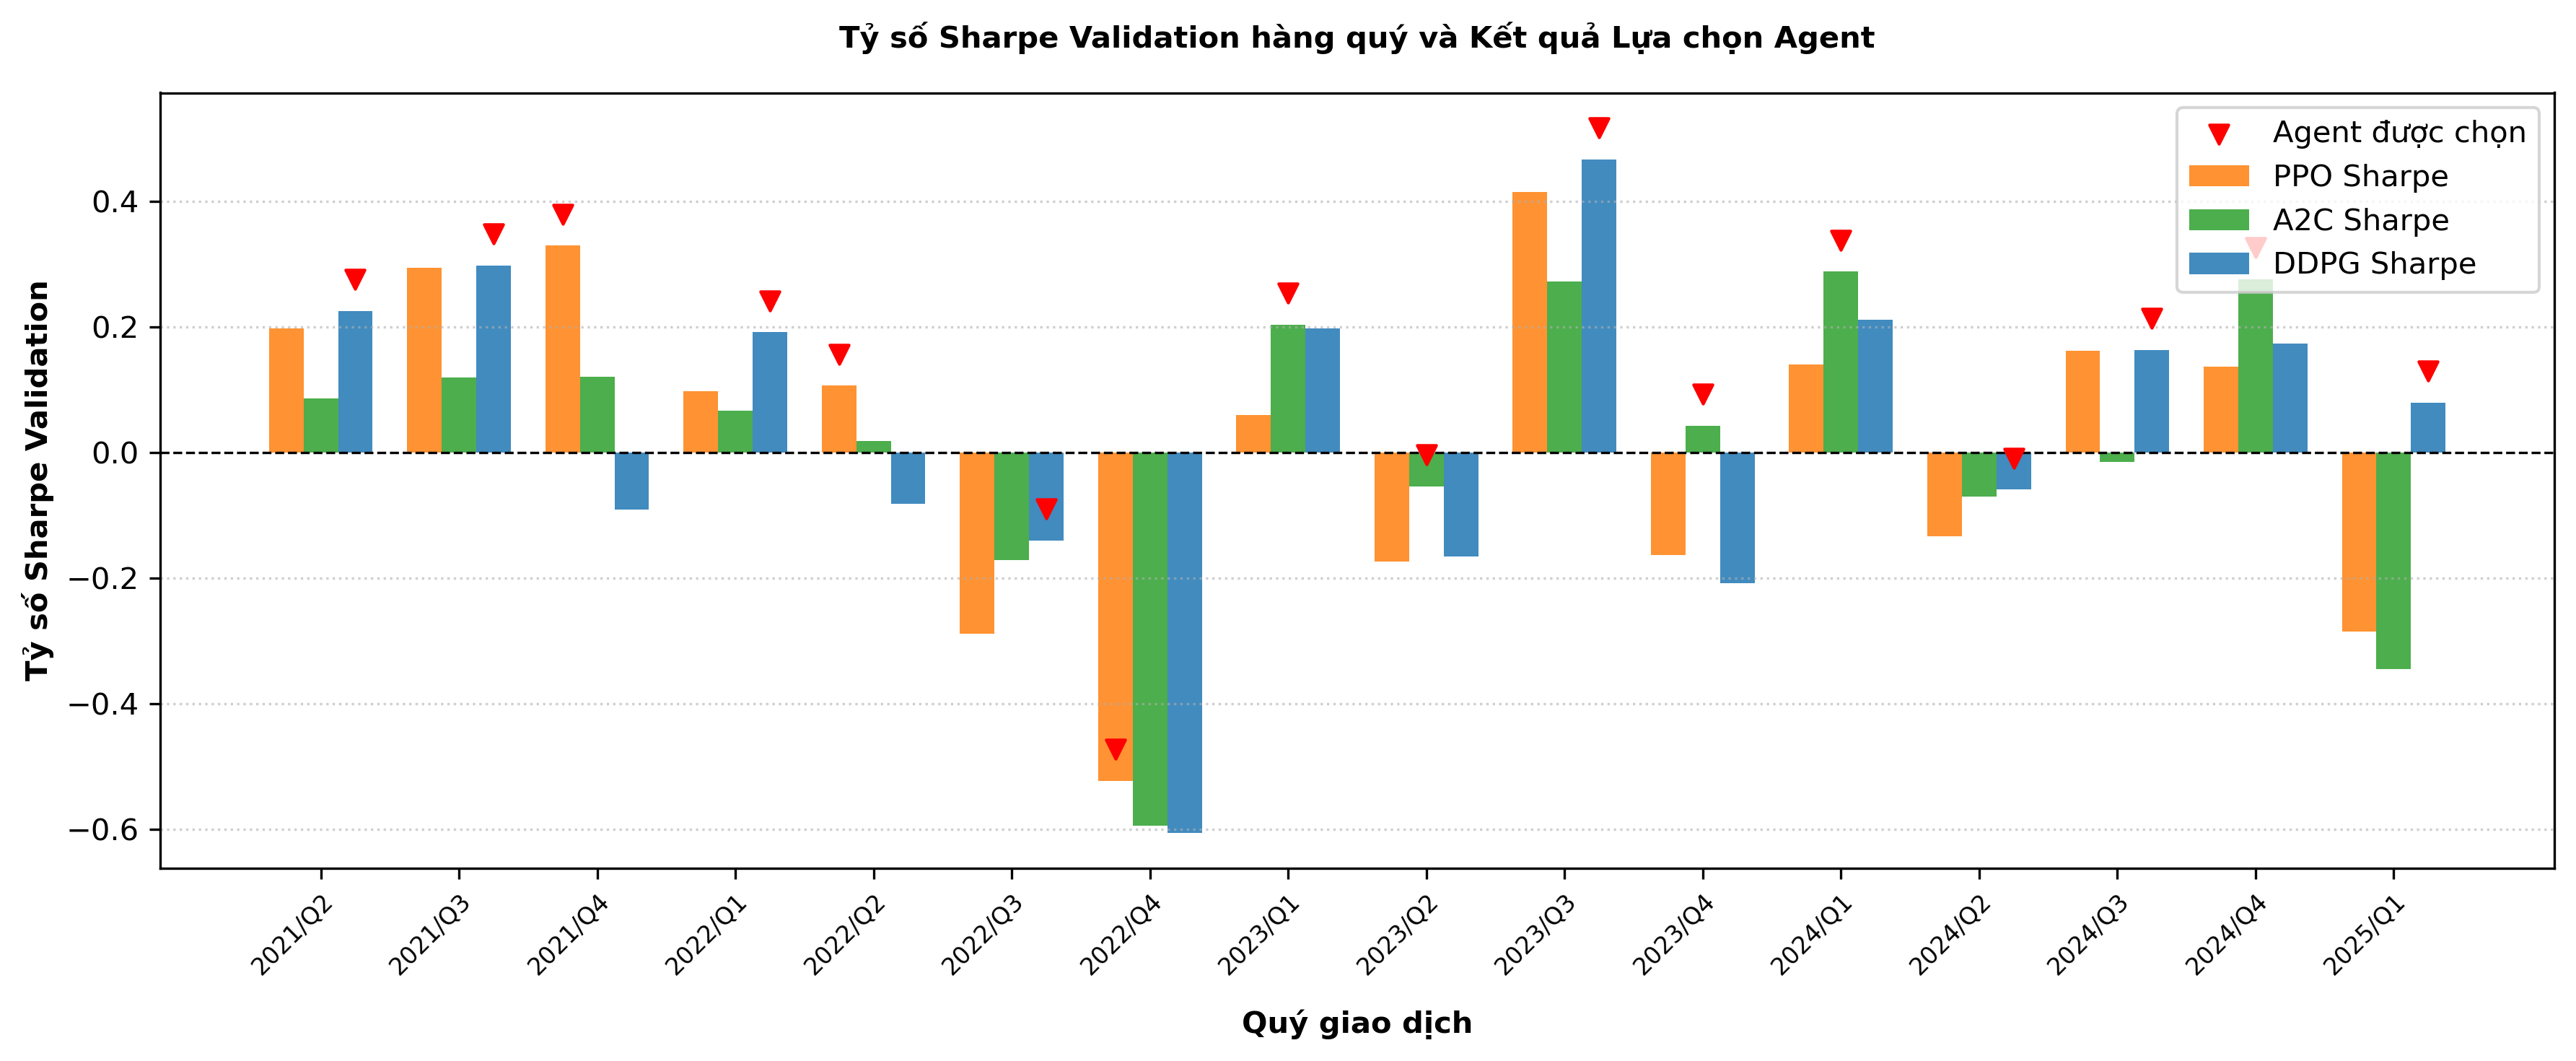
\includegraphics[width=\textwidth]{../figs/validation_sharpe_bar.png}
    \end{column}
    \begin{column}{0.36\textwidth}
      \centering
      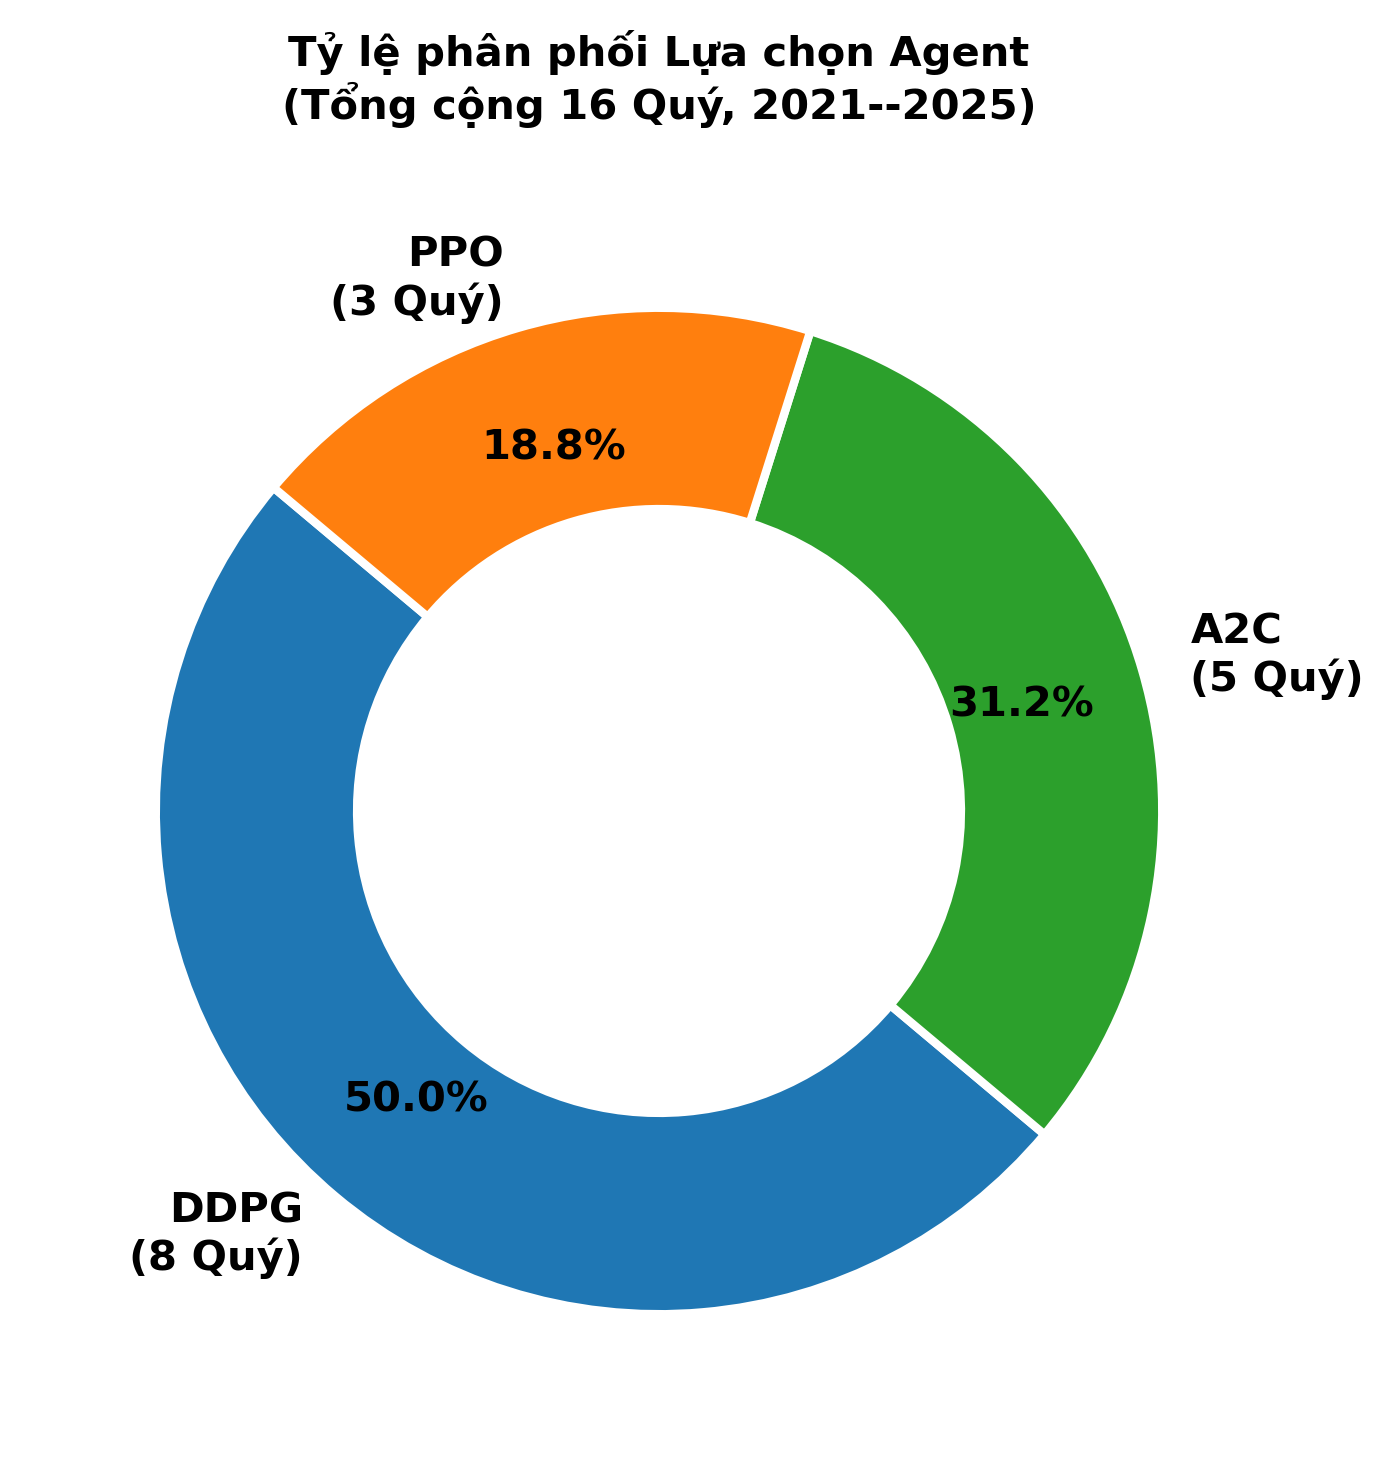
\includegraphics[width=\textwidth]{../figs/agent_selection_donut.png}
    \end{column}
  \end{columns}
\end{frame}

% --- Slide 24: Kết quả Thực nghiệm ---
\begin{frame}{Kết quả Thực nghiệm (2021--2025)}
  \begin{columns}[c]
    \begin{column}{0.54\textwidth}
      \begin{table}[h]
        \centering
        \caption{Kết quả kiểm thử thực tế (2021-01-04 đến 2025-05-30)}
        \scriptsize
        \setlength{\tabcolsep}{3pt}
        \begin{tabular}{ccccc}
          \toprule
          \textbf{Chỉ số} & \textbf{A2C} & \textbf{PPO} & \textbf{DDPG} & \textbf{Ensemble} \\
          \midrule
          \textbf{LN lũy kế} & 21.32\% & 38.78\% & \textbf{49.66\%} & 35.90\% \\
          \textbf{LN năm} & 6.74\% & 10.07\% & \textbf{11.77\%} & 9.41\% \\
          \textbf{Độ biến động} & 19.49\% & 19.33\% & \textbf{18.30\%} & 18.57\% \\
          \textbf{Sharpe} & 0.3458 & 0.5212 & \textbf{0.6432} & 0.5066 \\
          \textbf{Max DD} & -27.51\% & -24.69\% & \textbf{-16.57\%} & -22.87\% \\
          \bottomrule
        \end{tabular}
      \end{table}
    \end{column}
    
    \begin{column}{0.44\textwidth}
      \begin{block}{Phân tích Số liệu thực nghiệm}
        \scriptsize
        \begin{itemize}
          \item \textbf{DDPG tối ưu nhất}: Vượt trội về cả lợi nhuận năm (\textbf{11.77\%}) và tỷ số Sharpe (\textbf{0.6432}).
          \item \textbf{Kiểm soát Drawdown}: DDPG hạn chế mức sụt giảm cực đại tốt nhất (\textbf{-16.57\%}), so với A2C (\textbf{-27.51\%}).
          \item \textbf{Ensemble cân bằng}: Đạt Sharpe \textbf{0.5066} và lợi nhuận lũy kế \textbf{35.90\%}, thể hiện tính ổn định tốt.
        \end{itemize}
      \end{block}
    \end{column}
  \end{columns}
\end{frame}

% --- Slide 24a (Mới): Biểu đồ So sánh Hiệu năng Thực nghiệm ---
\begin{frame}{Biểu đồ So sánh Hiệu năng Thực nghiệm (2021--2025)}
  \begin{columns}[c]
    \begin{column}{0.62\textwidth}
      \centering
      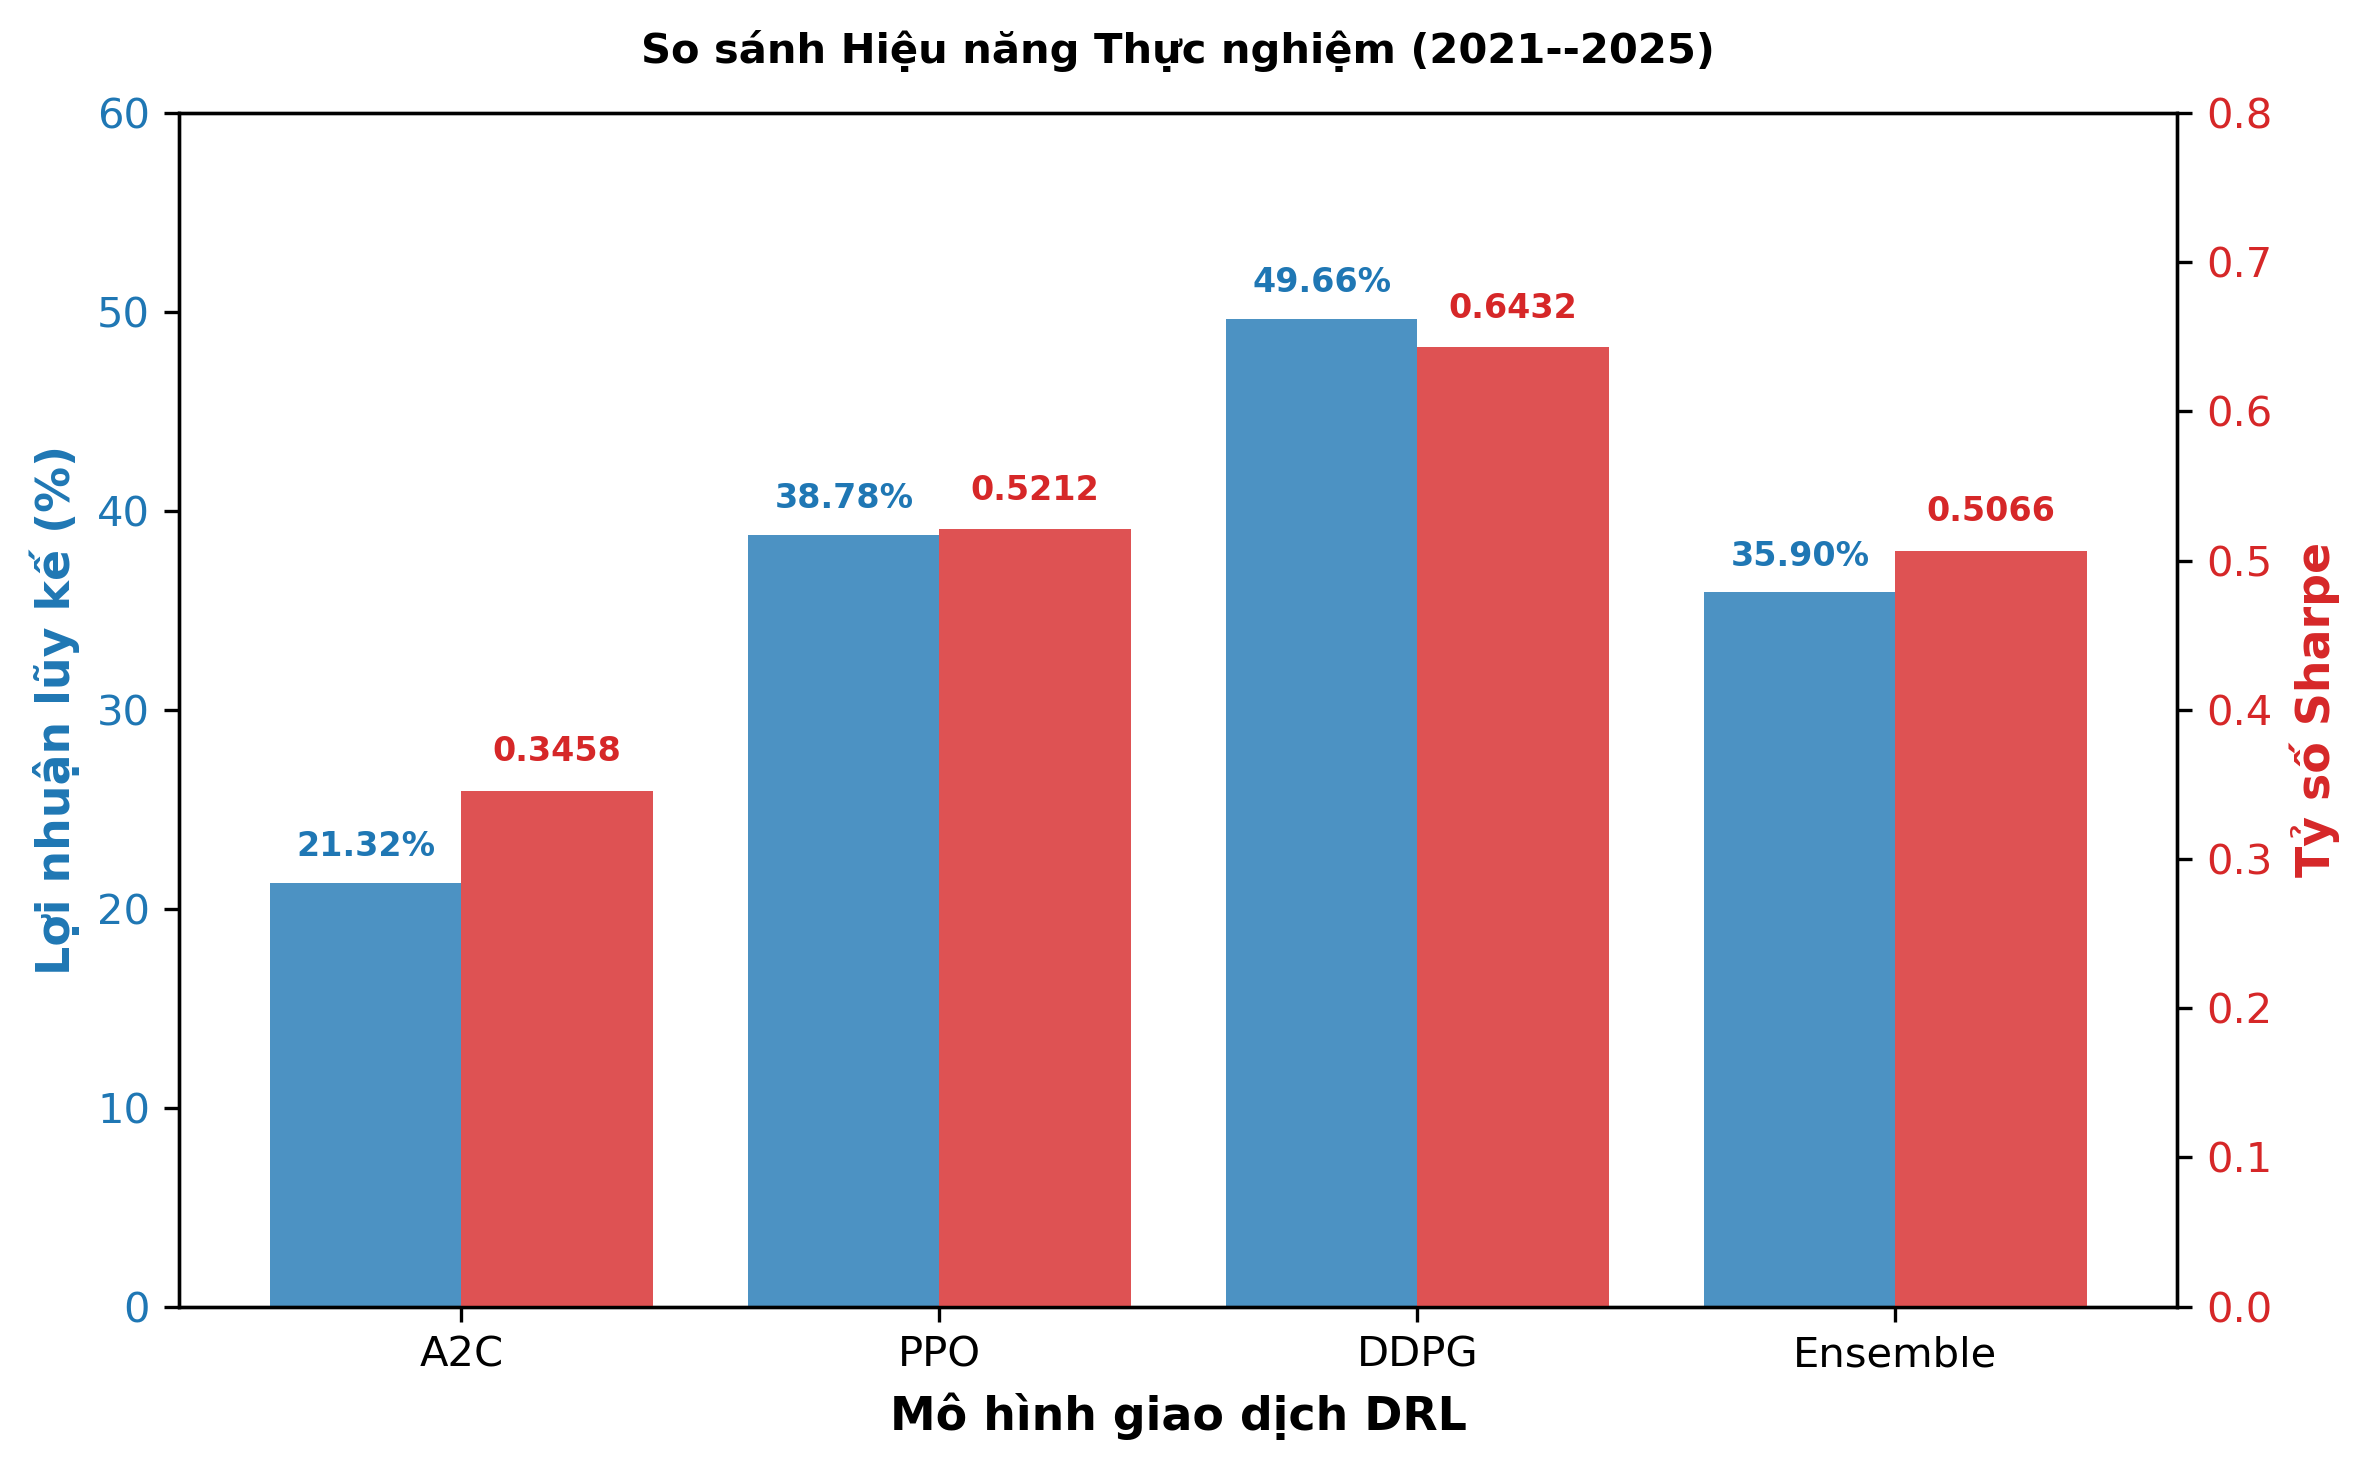
\includegraphics[width=\textwidth]{../figs/performance_comparison_bar.png}
    \end{column}
    \begin{column}{0.34\textwidth}
      \begin{block}{Nhận xét biểu đồ}
        \scriptsize
        \begin{itemize}
          \item \textbf{Lợi nhuận \& Sharpe}: Thứ tự hiệu năng đồng nhất giữa các tác tử: DDPG > PPO > Ensemble > A2C.
          \item \textbf{Vượt trội của DDPG}: Cột xanh (lợi nhuận) và đỏ (Sharpe) của DDPG đều cao nhất, chứng minh tính thích ứng xuất sắc.
        \end{itemize}
      \end{block}
    \end{column}
  \end{columns}
\end{frame}

% --- Slide 24b (Mới): Biểu đồ Lợi nhuận Lũy kế Thực nghiệm ---
\begin{frame}{Biểu đồ Lợi nhuận Lũy kế Thực nghiệm (2021--2025)}
  \begin{columns}[c]
    \begin{column}{0.65\textwidth}
      \centering
      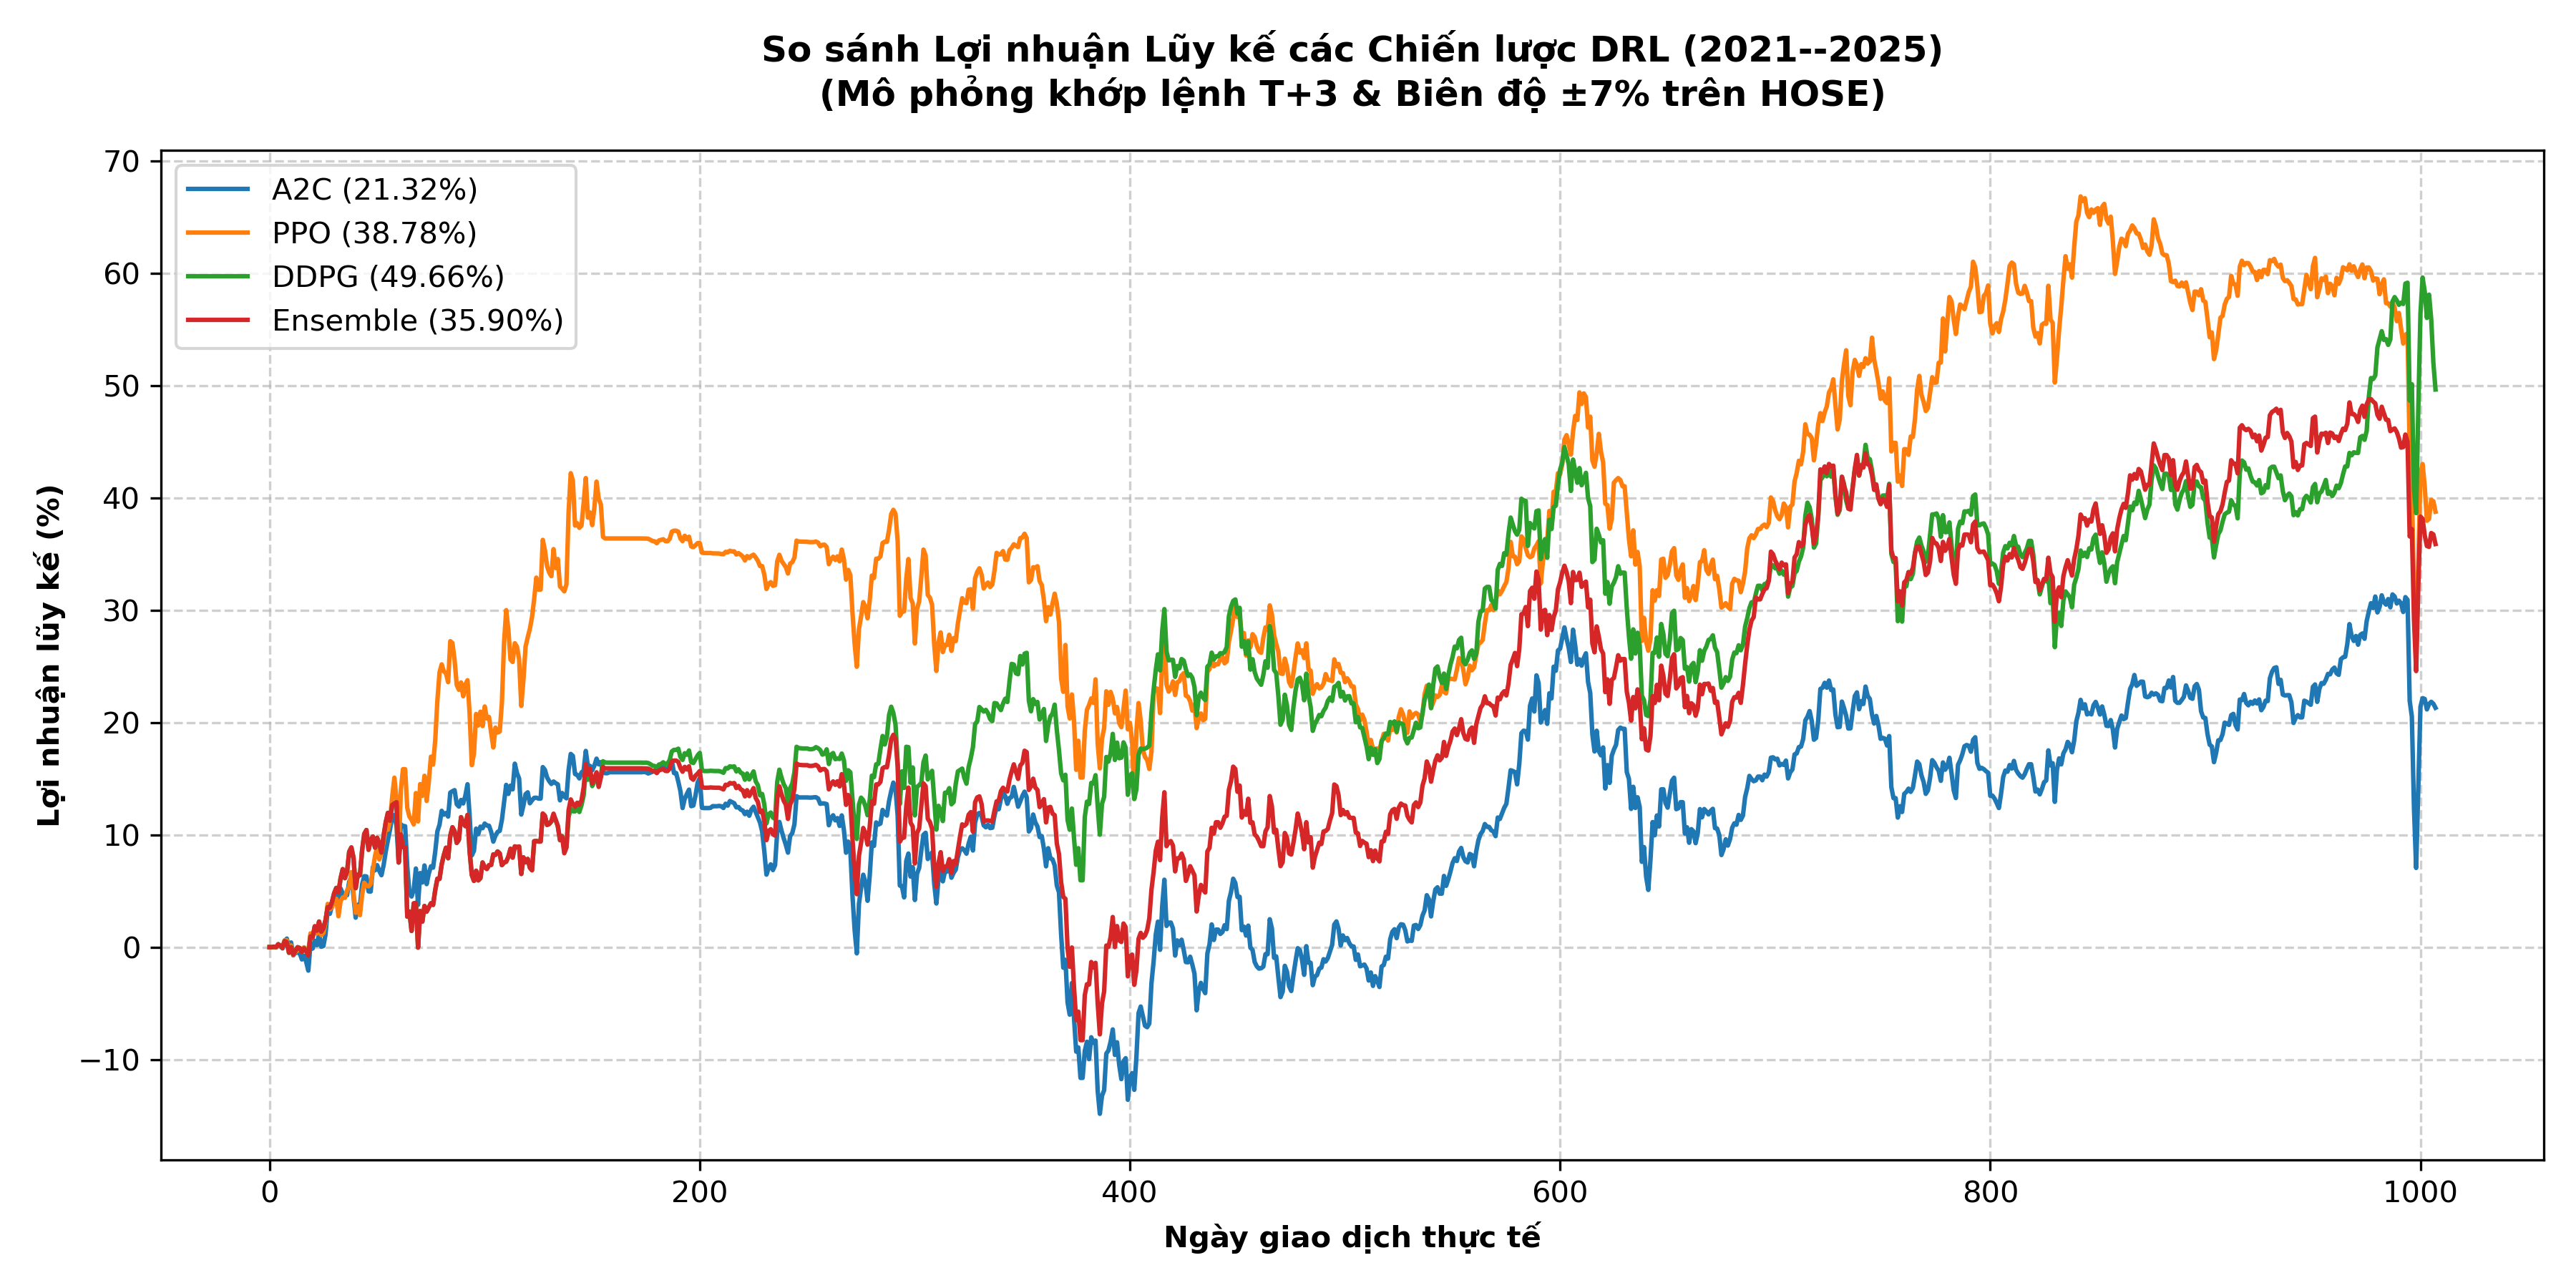
\includegraphics[width=\textwidth]{../figs/strategy_comparison.png}
    \end{column}
    \begin{column}{0.33\textwidth}
      \begin{block}{Nhận xét quan trọng}
        \scriptsize
        \begin{itemize}
          \item \textbf{DDPG dẫn đầu}: Đạt hiệu suất cao nhất và giữ khoảng cách ổn định nhờ tối ưu hóa liên tục.
          \item \textbf{PPO \& Ensemble}: Xu hướng biến động rất tương đồng nhau, bám sát nhau trong suốt chu kỳ.
          \item \textbf{A2C kém hiệu quả}: Bị tụt lại phía sau và gặp mức sụt giảm sâu trong năm 2022.
        \end{itemize}
      \end{block}
    \end{column}
  \end{columns}
\end{frame}

% --- Slide 24c (Mới): Biểu đồ Mức Sụt giảm Tài sản (Drawdown) ---
\begin{frame}{Biểu đồ Sụt giảm Tài sản (Drawdown) Thực nghiệm (2021--2025)}
  \begin{columns}[c]
    \begin{column}{0.65\textwidth}
      \centering
      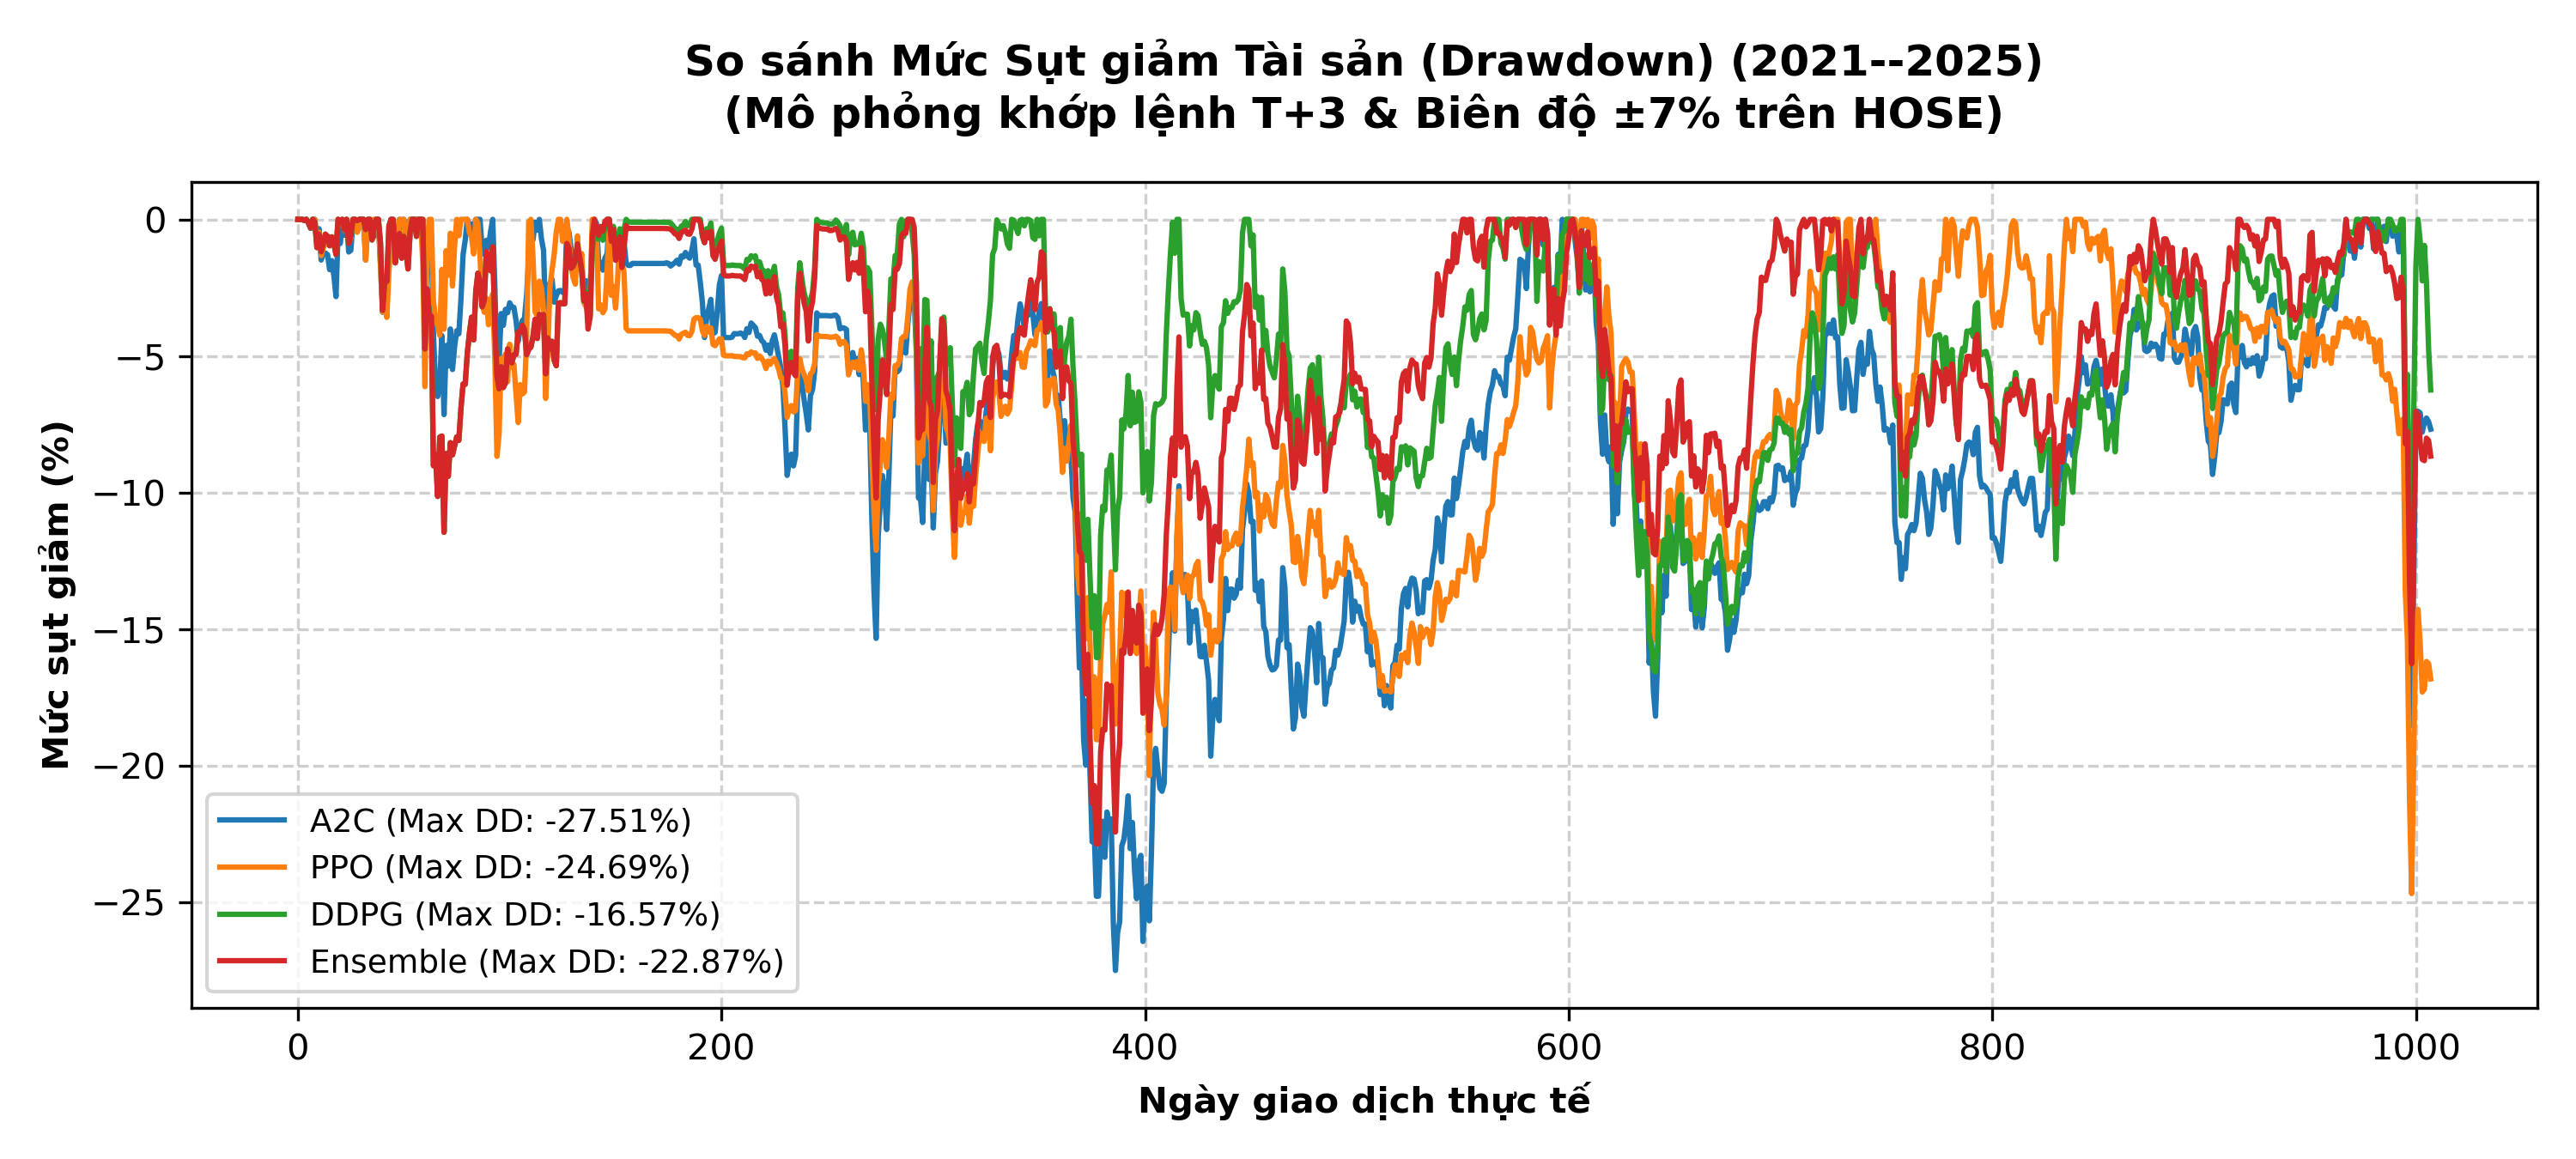
\includegraphics[width=\textwidth]{../figs/strategy_drawdown.png}
    \end{column}
    \begin{column}{0.33\textwidth}
      \begin{block}{Phân tích sụt giảm}
        \scriptsize
        \begin{itemize}
          \item \textbf{DDPG (Đen)}: Kiểm soát rủi ro xuất sắc, giữ mức sụt giảm cực đại thấp nhất (\textbf{-16.57\%}).
          \item \textbf{A2C (Đỏ)}: Chịu ảnh hưởng nặng nề nhất khi thị trường giảm sâu năm 2022 (\textbf{-27.51\%}).
          \item \textbf{Ensemble}: Giảm thiểu sụt giảm tốt hơn A2C nhờ phân bổ tài sản linh hoạt.
        \end{itemize}
      \end{block}
    \end{column}
  \end{columns}
\end{frame}

% --- Slide 25 (Mới): Phân tích Hiệu năng Ensemble & Chi phí ma sát ---
\begin{frame}{Phân tích Hiệu năng Ensemble \& Chi phí Ma sát}
  Mặc dù chiến lược Ensemble đạt hiệu năng tốt (\textbf{35.90\%} Sharpe \textbf{0.5066}), nó vẫn thấp hơn DDPG đơn lẻ (\textbf{49.66\%}) do hai yếu tố chính:
  \vspace{0.2cm}
  \begin{columns}[t]
    \begin{column}{0.48\textwidth}
      \begin{block}{Độ trễ lựa chọn (Selection Lag)}
        \begin{itemize}
          \item Ensemble chọn mô hình tốt nhất cho quý sau dựa trên Sharpe của quý trước (validation).
          \item Trong các giai đoạn thị trường đảo chiều nhanh (Uptrend sang Downtrend), mô hình tối ưu được chọn bị trễ pha so với xu hướng thực tế của quý kiểm thử.
        \end{itemize}
      \end{block}
    \end{column}
    
    \begin{column}{0.48\textwidth}
      \begin{alertblock}{Chi phí ma sát tái cơ cấu}
        \begin{itemize}
          \item Mỗi khi Ensemble chuyển đổi mô hình (ví dụ: A2C sang DDPG), danh mục tài sản bị tái cấu trúc lớn.
          \item Phí giao dịch thực tế ($0.1\%$) phát sinh liên tục trong quá trình chuyển đổi làm hao hụt lợi nhuận lũy kế so với việc nắm giữ mô hình DDPG ổn định.
        \end{itemize}
      \end{alertblock}
    \end{column}
  \end{columns}
\end{frame}

% --- Slide 26: Hiệu quả của chỉ số Turbulence ---
\begin{frame}{Hiệu quả Phòng vệ Khủng hoảng của Chỉ số Hỗn loạn}
  Chỉ số Turbulence tính toán dựa trên ma trận hiệp phương sai của 15 mã cổ phiếu HOSE đóng vai trò là một "hệ thống cảnh báo sớm" đắc lực:
  \vspace{0.3cm}
  \begin{columns}[t]
    \begin{column}{0.48\textwidth}
      \begin{block}{Khủng hoảng COVID-19 (Đầu năm 2020)}
        \begin{itemize}
          \item Giai đoạn dịch bệnh bùng phát khiến thị trường sụt giảm mạnh.
          \item Chỉ số Turbulence lập tức vượt ngưỡng phân vị 90.
          \item Kích hoạt chế độ phòng vệ: \textbf{Bán sạch cổ phiếu về tiền mặt}, tránh hoàn toàn cú giảm sập \textbf{33\%} của VN-Index.
        \end{itemize}
      \end{block}
    \end{column}
    
    \begin{column}{0.48\textwidth}
      \begin{block}{Khủng hoảng Trái phiếu Doanh nghiệp (2022)}
        \begin{itemize}
          \item Các vụ bắt bớ và thắt chặt dòng vốn gây ra hiện tượng mất thanh khoản diện rộng và call margin chéo.
          \item Turbulence phát hiện sự lệch pha nghiêm trọng trong phân phối lợi nhuận, \textbf{ngăn chặn các hành vi bắt đáy} rủi ro.
          \item Bảo vệ tối đa sự sụt giảm sâu của tổng tài sản ròng.
        \end{itemize}
      \end{block}
    \end{column}
  \end{columns}
\end{frame}

% --- Slide 26b (Mới): Biểu đồ biến động chỉ số Turbulence ---
\begin{frame}{Biểu đồ Biến động Chỉ số Turbulence (2021--2025)}
  \begin{columns}[c]
    \begin{column}{0.65\textwidth}
      \centering
      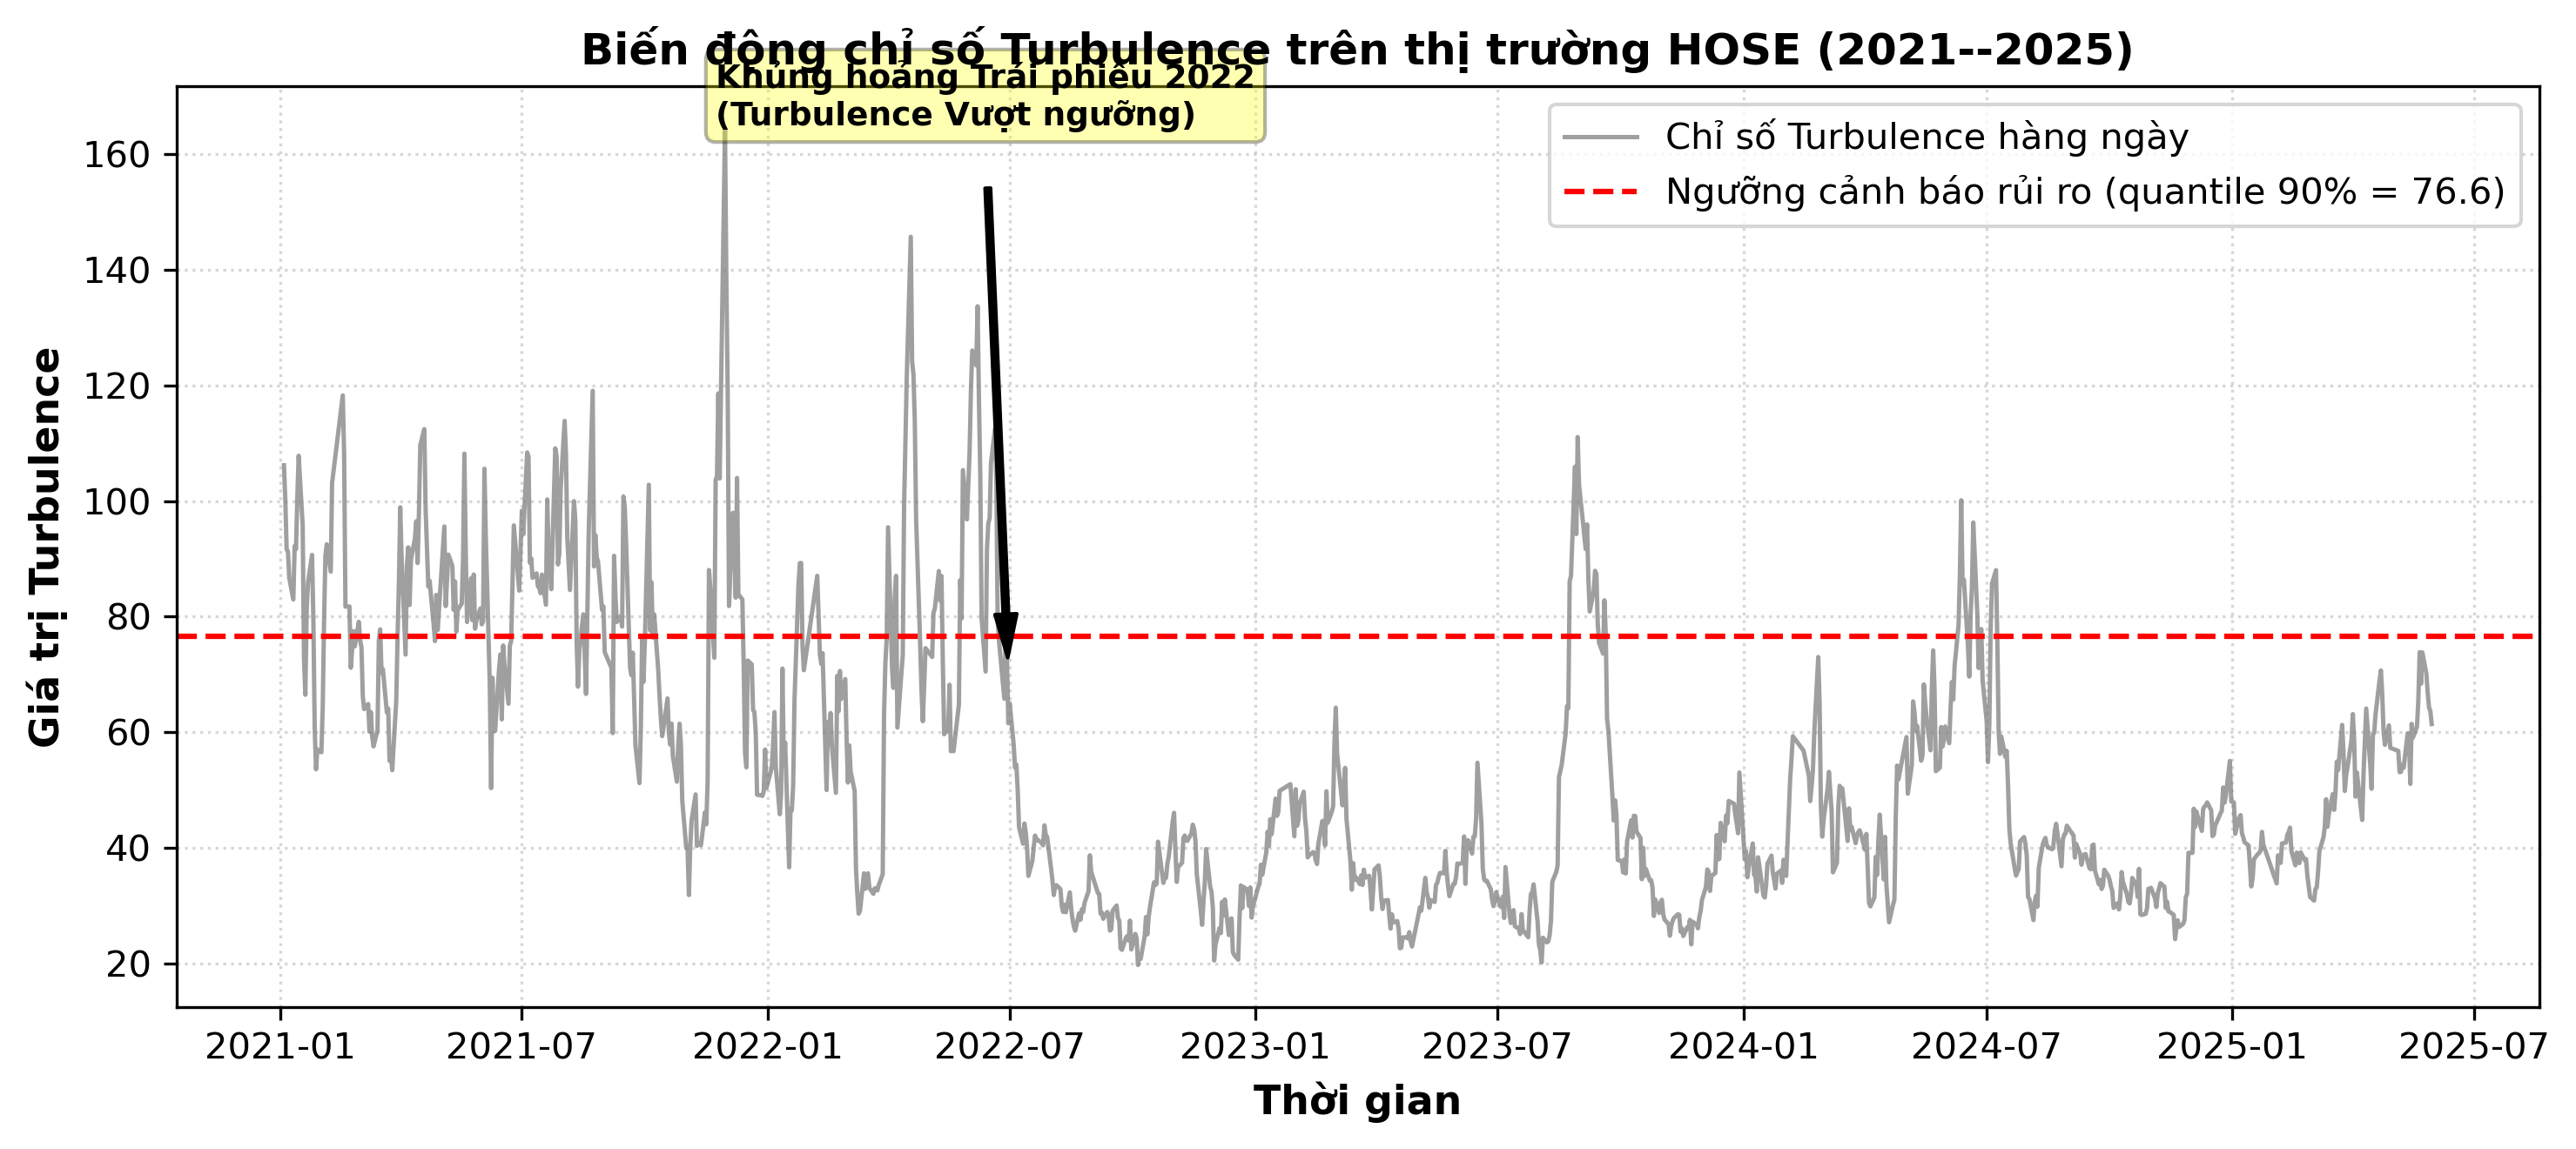
\includegraphics[width=\textwidth]{../figs/turbulence_index.png}
    \end{column}
    \begin{column}{0.33\textwidth}
      \begin{block}{Chỉ số Hỗn loạn}
        \scriptsize
        \begin{itemize}
          \item \textbf{Cảnh báo chính xác}: Vượt ngưỡng phân vị 90 (đường đỏ nét đứt) tại các điểm thị trường sụt giảm lớn (đặc biệt là năm 2022).
          \item \textbf{Cơ chế phòng vệ}: Chuyển danh mục đầu tư về tiền mặt giúp bảo vệ vốn hiệu quả trước các cú sốc vĩ mô.
        \end{itemize}
      \end{block}
    \end{column}
  \end{columns}
\end{frame}

% ==============================================================================
% PHẦN VIII: THẢO LUẬN & KẾT LUẬN
% ==============================================================================
\begin{frame}[plain,c]
  \setbeamercolor{background canvas}{bg=primary}
  \color{white}
  \centering
  \Huge \textbf{Phần VIII}\\
  \vspace{0.5cm}
  \Large \color{secondary} VIII. Thảo luận \& Kết luận
\end{frame}

% --- Slide 26: Thảo luận & Hạn chế ---
\begin{frame}{Thảo luận \& Các điểm điều chỉnh tại Việt Nam}
  \begin{block}{Sự điều chỉnh tối ưu cho thị trường Việt Nam}
    \begin{itemize}
      \item \textbf{Tinh giản danh mục ($D=15$)}: Đảm bảo tính liên tục của dữ liệu lịch sử, loại bỏ nhiễu từ các mã thiếu thanh khoản.
      \item \textbf{Hiệu chỉnh cách tính Turbulence}: Loại bỏ năm đầu tiên khỏi quá trình tính ngưỡng để tránh hạ thấp ngưỡng cảnh báo giả do các số 0 khởi động ma trận.
    \end{itemize}
  \end{block}
  \vspace{0.1cm}
  \begin{exampleblock}{Các ràng buộc thực tế đã được tích hợp thành công}
    \begin{itemize}
      \item \textbf{Mô phỏng chu kỳ thanh toán T+3}: Tiền bán chứng khoán được đưa vào hàng đợi chờ thanh toán và chỉ khả dụng để mua lại sau 3 ngày giao dịch.
      \item \textbf{Ràng buộc biên độ trần/sàn $\pm 7\%$ cứng}: Tự động chặn các hành động Mua (khi giá chạm trần) và Bán (khi giá chạm sàn) trong hàm bước của môi trường.
    \end{itemize}
  \end{exampleblock}
\end{frame}

% --- Slide 27: Kết luận & Hướng đi tương lai ---
\begin{frame}{Kết luận \& Hướng đi tương lai}
  \begin{columns}[t]
    \begin{column}{0.48\textwidth}
      \begin{block}{Kết luận}
        \begin{itemize}
          \item Khung DRL Ensemble đa Agent hoàn toàn có khả năng chuyển giao và ứng dụng thực tế hiệu quả trên thị trường chứng khoán Việt Nam.
          \item Kết hợp giữa mô hình DRL tối ưu vị thế liên tục và chỉ số quản trị rủi ro vĩ mô mang lại sự cân bằng hoàn hảo giữa lợi nhuận và an toàn tài sản.
        \end{itemize}
      \end{block}
    \end{column}
    
    \begin{column}{0.48\textwidth}
      \begin{exampleblock}{Hướng đi tương lai}
        \begin{itemize}
          \item Tích hợp các mô hình DRL tiên tiến hơn như \textbf{SAC} (Soft Actor-Critic) hoặc \textbf{TD3} (Twin Delayed DDPG) để tăng tốc độ hội tụ.
          \item Tối ưu hóa thời gian thực và rút ngắn chu kỳ tái cân bằng để giảm thiểu độ trễ lựa chọn (\textit{Selection Lag}) của Ensemble.
          \item Tích hợp thêm các biến vĩ mô (tỷ giá, lãi suất liên ngân hàng) và tâm lý mạng xã hội làm đầu vào trạng thái.
        \end{itemize}
      \end{exampleblock}
    \end{column}
  \end{columns}
\end{frame}

% --- Slide 28: Lời cảm ơn ---
\begin{frame}[plain,c]
  \setbeamercolor{background canvas}{bg=primary}
  \color{white}
  \centering
  \Huge \textbf{Trân trọng cảm ơn!}\\
  \vspace{0.5cm}
  \Large Q\&A - Thảo luận đóng góp ý kiến
\end{frame}

\end{document}
